%%
%% This is file `thesis-ex.tex',
%% generated with the docstrip utility.
%%
%% The original source files were:
%%
%% uiucthesis2009.dtx  (with options: `example')
%% 

%% Package and Class "uiucthesis2009" for use with LaTeX2e.
\documentclass[edeposit,fullpage, centerchapter]{uiucthesis2009}
\usepackage{graphicx}
\usepackage{amsmath}
\usepackage{fancyhdr}
\lhead{}
\pagestyle{fancy}


\begin{document}

\title{DIRECT ENERGY LANDSCAPE SAMPLING OF THE HOMOGENEOUS NUCLEATION AND CRYSTAL GROWTH OF A MODEL LIQUID}
\author{Nathan Peller Walter}
\department{Nuclear, Plasma, and Radiological Engineering}

\msthesis
\advisor{Yang Zhang}
\degreeyear{2016}
\committee{Assistant Professor Yang Zhang, Adviser\\Professor Brent Heuser}

\maketitle

\frontmatter

%% Create an abstract that can also be used for the ProQuest abstract.
%% Note that ProQuest truncates their abstracts at 350 words.
\begin{abstract}
%% ABSTRACT Material
A material's properties can be effected greatly by the method of synthesis of the material.  The first step in the synthesis of any material is the nucleation of the material's phase.  Nucleation and crystal growth are understood to be activated processes involving the crossing of free-energy barriers. Attempts to capture the entire crystallization process over long timescales with molecular dynamic simulations have met major obstacles because of the temporal constraints of molecular dynamics. Herein, we circumvent this temporal limitation by using an improved metadynamics method based on the adaptive basin-climbing algorithm to directly sample the potential-energy landscape of a monotonic, model-liquid Argon system. The algorithm biases the system to evolve from a liquid-like structure towards an FCC crystal structure through inherent structures.  Compared to other computational techniques, our method requires no assumptions about the shape, size, or thermodynamics properties of the critical crystal nucleus, and does not require a nucleation seed to simulate the growth process.  Consequently, the sampled timescale is macroscopically long, magnitudes longer than molecular dynamics simulations.  Thus, we observe that the formation of a crystal involves two processes, each with a unique temperature-dependent energy barrier. One barrier corresponds to the creation of a crystal nucleation site; the other barrier corresponds to the crystal growth. We find the two processes dominate in different temperature regimes.  Further, we provide empirical evidence for the non-monotonic temperature dependence of the nucleation energy barrier and the nucleation rate.  Then, we also use metadynamics on a fragile glass forming system, and compare the landscape and timescale of the fragile glass former to the good crystal former.  The stark difference in landscapes provides an energy landscape explanation for the nucleation process.  The success of this method on a model liquid system is encouraging for elucidating the crystallization of more complex systems. 
\end{abstract}

%% Create a dedication in italics with no heading, centered vertically
%% on the page.
\begin{dedication}
\input{./include/dedication}
\end{dedication}

%% Create an Acknowledgements page, many departments require you to
%% include funding support in this.
\chapter*{Acknowledgments}
First, I would like to thank my family, my friends, and my roommates for always supporting me and listening to my complaints when I was stressed and tired.  I would also like to thank my lab mates Abhishek Jaiswal and Zhikun Cai for their useful discussions of results, for patiently teaching me when I first joined the group, and especially for helping me with codes and scripts.  

Most importantly, I would like to thank Professor Yang Zhang for his clairvoyant guidance, insightful mentoring, and patient help during this project.  He has been invaluable to this work as well as my development as a graduate student.  

Lastly, I would like to acknowledge the Nuclear Regulatory Commission (NRC) for providing me with the fellowship that has funded me during the extent of this research.

%% The thesis format requires the Table of Contents to come
%% before any other major sections, all of these sections after
%% the Table of Contents must be listed therein (i.e., use \chapter,
%% not \chapter*).  Common sections to have between the Table of
%% Contents and the main text are:
%%
%% List of Tables
%% List of Figures
%% List Symbols and/or Abbreviations
%% etc.

\tableofcontents
\listoftables
\listoffigures

%% Create a List of Abbreviations. The left column
%% is 1 inch wide and left-justified
\chapter{List of Abbreviations}
\begin{symbollist*}
\item[BOP] Bond orientational order parameter
\item[PEL] Potential Energy Landscape
\item[MD] Molecular Dynamics
\item[MC] Monte Carlo
\item[MTD] Metadynamics
\item[LJ] Lennard-Jones 
\item[BCC] Body centered cubic
\item[FCC] Face centered cubic
\item[HCP] Hexagonal close packing
\item[liq] Liquid State
\item[IE] Inherent Energy
\item[CNT] Classical Nucleation Theory
\item[NVT] Constant number, volume, and temperature 
\item[NPT] Constant number, pressure, and temperature
\end{symbollist*}

%% Create a List of Symbols. The left column
%% is 0.7 inch wide and centered
\chapter{List of Symbols}

\begin{symbollist}[0.7in]
\item[$\bar{q}_6$] Sixth-order, first nearest-neighbor averaged, bond orientational order parameter 
\item[$T_m$] Melting temperature
\item[$T_g$] Glass transition temperature
\item[$\phi$] Penalty Potential Energy Function
\item[$\alpha$] Newton's Steepest Descent Step Size
\item[$\delta$] Force Step Size
\end{symbollist}

\mainmatter
\chapter{Introduction}
Matter is described by its phase composition, where a phase is defined as a region in which the physical properties of the system are uniform.  These physical properties include density, structure, specific heat, conductivity, etc \cite{HANSEN2006v}.  Typically, a substance will exhibit similar phases for a range of thermodynamic variables, such as temperature, pressure, or volume.  A collection of state points in which the substance exhibits similar properties is defined as a state of matter, i.e. gas, liquid, solid, and can be summarized by a phase diagram \cite{HANSEN2006v}.  A phase diagram's two axis are relevant thermodynamics variables such as temperature, pressure, density, volume, etc.  Figure \ref{phase diagram} shows an example of a pressure-temperature phase diagram, which divides the regions of the pressure-temperature space based on thermodynamic properties of the substance \cite{EGELSTAFF}. 

\begin{figure}[h]
	\centering
	\includegraphics[width = .5\textwidth]{./Figures/Introduction/phase_diagram.png}
	\caption[An example of a schematic phase diagram.  There are phase regions, solid, liquid, gas, and a region known as supercritical fluid (liquid and gas become indistinguishable), each with a corresponding phase boundary dividing them.  A black x represents a system in a stable phase, and a black o represents a system in a metastable phase.]{An example of a schematic phase diagram.  There are phase regions, solid, liquid, gas, and a region known as supercritical fluid (liquid and gas become indistinguishable), each with a corresponding phase boundary dividing them.  A black x represents a system in a stable phase, and a black o represents a system in a metastable phase.\cite{EGELSTAFF}}
	\label{phase diagram}
\end{figure}

From Figure \ref{phase diagram}, the stable phase of a substance can be determined based on the substance's temperature and pressure.  The different phases are divided by coexistence lines, which indicate a state point in which both phases can simultaneously exist.  When the thermodynamic properties of a substance crosses a coexistence line, a phase transition may occur, in which the substance's physical properties change from one phase to another \cite{askeland2011the}.  Across these lines, there is a discontinuous change in physical properties such as density or entropy \cite{EGELSTAFF}.  However, this transition between phases can also be suppressed giving rise to the existence of supercooled or superheated phases \cite{askeland2011the}.  For example, a liquid substance cooled passed the coexistence line can exists as a metastable, supercooled liquid for various lengths of time.  This phase is considered metastable because the solid phase is knowingly more stable (the free energy of the metastable phase is greater than the stable phase).  However, there is a significant time for the substance to transition to the solid phase from the supercooled liquid phase \cite{Sear2016}.  This is shown in Figure \ref{phase diagram} by the black x's and o's.  The system begins as a stable liquid system, and is cooled beyond the coexistence line resulting in a supercooled liquid.

Once the coexistence line is reached or passed, the transition from one phase to another is initiated by the nucleation process.  Nucleation is the formation of a new phase or structure by re-organization within a preexisting phase or structure.  Nucleation can occur in two distinct manners.  First, known as heterogeneous nucleation, this is nucleation occurring along a container surface, an impurity, or a defect in the system \cite{Schmelzer2005}.  For example, heterogeneous nucleation occurs in the condensation along a water bottle edge.  The second form of nucleation is homogeneous nucleation, or nucleation that occurs in the bulk of a system, in the absence of impurities or surfaces \cite{Schmelzer2005}.  Heterogeneous nucleation occurs preferentially to its homogeneous counterpart, because the surface or impurity provide a seed to start the nucleation process \cite{Schmelzer2005}.  Nucleation results in a seed of the new phase.  This new phase, because it is energetically more stable, grows throughout the system until the new phase is ubiquitous in the system \cite{Schmelzer2005}.  As a result, there are two key rates in the formation of the new phase from a supercooled liquid phase, the nucleation rate and the growth rate, which are displayed in Figure \ref{overall_rates} \cite{barrett1973the}.

\begin{figure}[h]
	\centering
	\includegraphics[width = .5\textwidth]{./Figures/Introduction/overall_rates.pdf}
	\caption[The theoretical nucleation, crystal growth rate, and the overall crystallization rate plotted versus temperature between the melting temperature, $T_m$, and the glass transition temperature, $T_g$.  The figure shows that crystal growth rates are larger at low subcooling because diffusion rates are higher at higher temperatures.  Similarly, the nucleation rate is higher at greater subcooling.  We assume that the overall rate for crystallization is the product of the two rates.]{The theoretical nucleation, crystal growth rate, and the overall crystallization rate plotted versus temperature between the melting temperature, $T_m$, and the glass transition temperature, $T_g$.  The figure shows that crystal growth rates are larger at low subcooling because diffusion rates are higher at higher temperatures.  Similarly, the nucleation rate is higher at greater subcooling.  We assume that the overall rate for crystallization is the product of the two rates. \cite{barrett1973the}\cite{Cavagna2009}}
	\label{overall_rates}
\end{figure}

Figure \ref{overall_rates} shows the two rates involved in crystal formation in a supercooled liquid, the nucleation rate and the crystal growth rate \cite{barrett1973the}.  The figure also shows the overall crystallization rate, which is the product of the nucleation and crystal growth rates.  The crystal growth and nucleation rates are shown to be monotonic as a function of temperature.  The crystal growth rate is low at high subcoolings because at low temperatures near the glass transition temperature, the dynamics of atoms is extremely slow.  As a result, atoms rarely move enough to combine with the nucleation site.  As the temperature is increased, the growth rate increases as the diffusion rate increases.  Conversely, the nucleation rate is low at low subcoolings, because fast diffusion rate leads to nucleation sites to dissipate before growth can begin.  As the temperature decreases, the nucleation rate increases because time for a nucleation site to dissipate decreases as dynamics slow.  Thus, the crystal growth rate has a maximum at the melting temperature, and the nucleation rate has a maximum at the glass temperature.  The overall crystallization rate is considered to be the product of the nucleation rate and crystal growth rate.  The overall crystallization rate has a maximum at an intermediate temperature between the melting temperature and glass transition temperature.  These results are shown in Figure \ref{overall_rates}.   The key feature predicted by theory is that different rates dominate in different temperature regimes, and the overall rate is non-monotonic.  Despite great effort devoted to the topic of nucleation, a complete understanding of the nucleation process from an experimental or computational approach is still lacking due to great difficulty in capturing the entire process.  

Experiments and simulations alike are very difficult to perform on the topic of nucleation, because nucleation is stochastic, transient, and atomic scale \cite{ReintenWolde1996}.  While experimental probes to capture atomic scale events exists, multiple nucleation sites often develop during experiments, and the deconvolution of the multiple nucleation events is difficult \cite{ReintenWolde1996}.  Similarly, traditional computational techniques such as molecular dynamics are limited in the timescales accessible.  Molecular dynamics is limited to the microsecond timescale, and the average time for a nucleation event to occur in a molecular dynamics simulation is beyond seconds.  It is the goal of this thesis to elucidate the true nature of the crystal growth rate and nucleation rate via metadynamics simulations.

Despite efforts to study nucleation experimentally, computationally, and theoretically, a complete understanding of the nucleation process of any phase transition is still incomplete \cite{Sanz2013}.  Understanding nucleation is an essential component to fully understand phase behavior in substances \cite{Reguera2013}.  The nucleation process influences the final crystal structure of substances with multiple polymorphs in the crystal phase \cite{Reguera2013}.  For example, nucleation can elucidate the origin of water freezing to one of seventeen different polymorphs at different state points \cite{Sanz2013}.  On the other hand, understanding the nucleation process can also provide new insight to the glass formation process.  Particularly, a complete understanding of nucleation may provide information about the origin of strong versus fragile glass formers, or the origin of good glass formers versus poor glass formers.  Nucleation also determines a material's transition from one crystal structure to another, which is of importance in electrical engineering.  Thus, an understanding of nucleation can provide insight on how to better predict and control the creation of materials.  Because the understanding of nucleation is essential to many fields of science and engineering, many nucleation theories have been proposed, the prevalent theory being classical nucleation theory.

Nucleation is traditionally described by classical nucleation theory (CNT) \cite{Sear2016}.  Classical nucleation theory assumes nucleation occurs via random density fluctuations resulting in nucleation sites of various size \cite{Sear2016}.  These sites will either collapse on itself or grow throughout the system depending on the size of the site.  The formation rate of these sites is estimated by the free energy barrier preventing the creation of these sites.  Classical nucleation estimates this free energy barrier with macroscopic quantities of the system.  Classical nucleation has been used alongside MD simulations \cite{Chkonia2009}.  CNT and MD has shown some success, but CNT is limited in its accuracy.  Many believe the short comings of CNT results from the approximations made to calculate the free energy barrier \cite{Chkonia2009}.  As a result, the goal of this thesis is to use metadynamics simulations to better estimate the free energy barrier involved in the nucleation process.

The remainder of this thesis will discuss our recent results on the homogeneous nucleation and crystal growth using metadynamics simulations to directly sample the energy landscape.  In chapter 2, we discuss classical nucleation theory, the prevailing method of explaining nucleation for decades, and discuss some of the pitfalls of the method.  In chapter 3, we discuss the metadynamics method used to directly sample the energy landscape as nucleation and crystal growth occur.  In chapter 4, the results of the metadynamics simulation are discussed.  In chapter 5, we discuss relevant differences between good crystal formers and good glass formers as shown by the energy landscape.  Lastly, in chapter 6, we summarize relevant conclusions and possible future work.  In the appendix section, honorable mentions are made to projects that support this research.

\chapter{Classical Nucleation Theory}
In 1877, and extended in 1926 by Volmer and Weber, Gibbs originally developed classical nucleation theory (CNT) for liquid formation in supercooled vapor \cite{debenedetti1996metastable}.  The theory was later extended to crystal formation in supercooled liquids \cite{debenedetti1996metastable}.  Gibbs theorized that, in order for a new phase to form in a bulk phase, a free energy barrier must be overcome for the creation of a nucleus site of the new phase.  Classical nucleation theory was the first framework to argue that the kinetic rates involved in nucleation depended on the exponential of a free energy activation barrier \cite{debenedetti1996metastable}.  This idea is pictorially displayed in Figure \ref{CNT} for the formation of a crystal in a bulk liquid.  

\begin{figure}[h]
	\centering
%	\includegraphics[width = .7\textwidth]{./Figures/cnt.pdf}
	\includegraphics[width = .5\textwidth]{./Figures/CNT/nucleation.png}
	\caption[Figure to show a schematic drawing of classical nucleation theory.  The figure shows the prevalent idea behind classical nucleation: nucleation is dominated by a single free-energy barrier that requires an activated event to overcome.  The figure shows to the left of the barrier the system is in the liquid phase, at the top of the barrier a critical nucleus site is formed of the crystal phase, and to the right is the fully developed crystal phase.  Generally, if a nucleation site as large as the critical size is created, the crystal phase will become ubiquitous in the system, but if the nucleation site is smaller, the liquid phase will remain ubiquitous.]{Figure to show a schematic drawing of classical nucleation theory.  The figure shows the prevalent idea behind classical nucleation: nucleation is dominated by a single free-energy barrier that requires an activated event to overcome.  The figure shows to the left of the barrier the system is in the liquid phase, at the top of the barrier a critical nucleus site is formed of the crystal phase, and to the right is the fully developed crystal phase.  Generally, if a nucleation site as large as the critical size is created, the crystal phase will become ubiquitous in the system, but if the nucleation site is smaller, the liquid phase will remain ubiquitous. \cite{debenedetti1996metastable}}
	\label{CNT}
\end{figure}

Figure \ref{CNT} shows a schematic drawing of the CNT framework \cite{debenedetti1996metastable}.  The figure shows that a system begins in a high energy amorphous state, and is separated from the stable crystal state by a large energy barrier \cite{debenedetti1996metastable}.  This barrier represents the energy cost for the system to enter a two phase state \cite{debenedetti1996metastable}.  CNT argues that a system in the absence of surfaces and impurities will under go random density fluctuations, resulting in sites of the more stable phase \cite{debenedetti1996metastable}.  If the new phase site is sufficiently large, the system will without bounds transition to the new phase.  However, if the site is not sufficiently large, the site will collapse back to the original phase.  CNT argues that nucleation is an activated process.  In this chapter, we will show how CNT approximates the height of this energy barrier and utilizes the barrier to estimate the nucleation rate.  Next, we will present some promising results employing CNT.  Lastly, discussion of the short comings of the framework, and how the theory can be improved will be presented.

\section{Estimating the Energy Barrier}
In the original theory, a liquid phase nucleation site develops in a bulk supercooled vapor \cite{mutaftschiev2001atomistic}.  In this theory, the nucleus is assumed to be spherical in shape and to be much larger than the atomic dimensions of the material (the radius of the nucleus is assumed larger than a few molecular diameters).  As a result of a new phase, an interface develops between the two phases, a liquid-vapor phase in the original theory.  Because of the aforementioned assumptions, this interface is treated macroscopically, despite being a microscopic feature.  Therefore, when a nucleation site forms, there is a free-energy penalty for the formation of the nucleation site, due to the introduction of this interface.  By assuming the interface can be treated macroscopically, the interface free energy is calculated by the surface tension of the new phase \cite{mutaftschiev2001atomistic}.
\begin{equation}
	\Delta G_{i} = A\gamma 
\end{equation}
where $A$ is the area of the nucleation site, and $\gamma$ is the surface tension of the liquid.

On the other hand, there is also a free energy difference from the creation of a new phase.  The free energy of the formation of a new phase is calculated from the chemical potential of the two phases \cite{mutaftschiev2001atomistic}.  Each phase has a chemical potential, $\mu$.
\begin{equation}
	\Delta G_{f} = V\rho\Delta \mu
\end{equation}
where $V$ is the volume of the nucleation site, $\rho$ is the atomic density, and $\Delta \mu$ is the difference in the chemical potential defined as
\begin{equation}
	\Delta \mu = \mu_{new} - \mu_{old}
\end{equation}
where $new$ and $old$ indicate the nucleation phase and the bulk phase, respectively.

Because the nucleation site is assumed spherical the area and the volume of the nucleation site is known as
\begin{equation}
	\begin{split}
		A &= 4\pi r^2\\
		V &= \frac{4}{3}\pi r^3 
	\end{split}
\end{equation}
where $r$ is the radius of the nucleation site \cite{mutaftschiev2001atomistic}.  Thus, the free energy barrier of nucleation as a function of nucleation site radius is determined by the following equation
\begin{equation}
	\Delta G(r) = \Delta G_{f}(r) + \Delta G_{i}(r) = \frac{4}{3}\pi r^3\rho \Delta \mu + 4\pi r^2\gamma
\end{equation}
This is pictorially displayed in Figure \ref{cnt_energy}.

\begin{figure}[h]
	\centering
	\includegraphics[width = .5\textwidth]{./Figures/CNT/cnt_energy.pdf}
	\caption[Gibbs free energy plotted as a function of nucleation cluster radius.  The blue line shows the energy change due to the formation of a nucleation site.  The orange line shows the energy change introduced by the interface between the two phases of the bulk phase and the nucleation site phase.  The yellow line shows the total of the formation energy and the interface energy.  The figure shows there is a critical value (maximum value) for the total of the two.  If the nucleation site has a radius less than the critical size, then the nucleation site will dissipate to reduce the Gibbs free energy of the system.  Comparatively, if the site is greater than the critical radius, then the nucleation site will preferentially grow to reduce the Gibbs free energy.]{Gibbs free energy plotted as a function of nucleation cluster radius.  The blue line shows the energy change due to the formation of a nucleation site.  The orange line shows the energy change introduced by the interface between the two phases of the bulk phase and the nucleation site phase.  The yellow line shows the total of the formation energy and the interface energy.  The figure shows there is a critical value (maximum value) for the total of the two.  If the nucleation site has a radius less than the critical size, then the nucleation site will dissipate to reduce the Gibbs free energy of the system.  Comparatively, if the site is greater than the critical radius, then the nucleation site will preferentially grow to reduce the Gibbs free energy. \cite{debenedetti1996metastable}}
	\label{cnt_energy}
\end{figure}

Figure \ref{cnt_energy} shows the free energy for the interface between the two phases, the formation of a new phase, and the total free energy change \cite{debenedetti1996metastable}.  In classical nucleation theory, while in equilibrium, a bulk material will undergo thermal and density fluctuations, which will lead to nucleation sites of the new phase \cite{mutaftschiev2001atomistic}.  These nucleation sites are assumed to have a certain radius.  If the radius is smaller than the critical radius, $r_{c}$, the site has not overcome the free energy barrier and the surface tension term will dominate causing the nucleation site to reduce back to the original phase \cite{mutaftschiev2001atomistic}.  Alternatively, if the nucleation site radius is equal to $r_{c}$ or larger than the site has overcome the free energy barrier and the formation energy will dominate \cite{mutaftschiev2001atomistic}.  As a result, since the new phase is energetically preferential at this temperature, the new phase will grow throughout the system \cite{debenedetti1996metastable}.  

The critical radius can simply be calculated by determining the derivative of the free energy of nucleation and setting the derivative to zero.
\begin{equation}
	\frac{d \Delta G(r)}{d r}\Bigg{|}_{r=r_{c}} = 4\pi\rho\Delta\mu r_{c}^2 + 8\pi \gamma r_{c} = 0
\end{equation}
Solving this for $r_{c}$, results in
\begin{equation}
	r_{c} = -\frac{2\gamma}{\rho\Delta\mu} = -\frac{2\gamma v}{\Delta\mu}
\end{equation}
where $v$ is the atomic specific volume \cite{Vehkamaki2006}.  The critical radius is negative here because $\Delta\mu$ is negative if the new phase is energetically favorable \cite{Vehkamaki2006}.  Thus,
\begin{equation}
\begin{split}
r_{c} = \frac{2\gamma v_l}{|\Delta\mu|} \quad \mu_{new} < \mu_{old} \\
r_{c} = -\frac{2\gamma v_l}{|\Delta\mu|} \quad \mu_{old} < \mu_{new} \\
\end{split}
\end{equation}
Thus, if the new phase is not energetically favorable, the critical radius is negative and, as a result, the new phase will never emerge \cite{Vehkamaki2006}.  

\begin{figure}[h]
	\centering
	\includegraphics[width = .5\textwidth]{./Figures/CNT/cnt_mu.pdf}
	\caption[Gibbs free energy plotted as a function of nucleation cluster radius.  The blue line is identical to the yellow line in Figure \ref{cnt_energy}.  When the difference in the chemical potential is negative (new phase is more stable), the Gibbs free energy takes the shape of the blue line.  However, if the difference in the chemical potential is positive (new phase is less stable), the Gibbs free energy takes the shape of the orange line, and the formation of the new phase is highly improbable.  If the difference in the chemical potential is zero, the two phases are in equilibrium, and neither phase will preferentially grow.]{Gibbs free energy plotted as a function of nucleation cluster radius.  The blue line is identical to the yellow line in Figure \ref{cnt_energy}.  When the difference in the chemical potential is negative (new phase is more stable), the Gibbs free energy takes the shape of the blue line.  However, if the difference in the chemical potential is positive (new phase is less stable), the Gibbs free energy takes the shape of the orange line, and the formation of the new phase is highly improbable.  If the difference in the chemical potential is zero, the two phases are in equilibrium, and neither phase will preferentially grow \cite{Vehkamaki2006}. }
	\label{cnt_mu}
\end{figure}

The chemical potential dependence is also pictorially displayed in Figure \ref{cnt_mu} \cite{Vehkamaki2006}.  This figure shows the total free energy for a nucleation site as function of nucleation site radius \cite{Vehkamaki2006}.  The figure shows that if the new phase is energetically favorable, $\mu_{new} < \mu_{old} $, there is an energy barrier that must be over come.  However, if the opposite is true, $\mu_{new} > \mu_{old}$, then the free energy increases to infinity as the radius goes to infinity, and as a result, the new phase will never develop in the system.  Lastly, if the new phase is assumed to be energetically favorable and the critical radius is positive, the free energy barrier can be computed as
\begin{equation}\label{G_critical}
\Delta G_{c} (r_{c}) = -\frac{4}{3}\pi \frac{8\gamma^3 v_l^3}{\Delta\mu^3}\frac{\Delta\mu}{v_l} + 4\pi\frac{4\gamma^2v_l^2}{\Delta\mu^2}\gamma = \frac{16\pi}{3}\frac{\gamma^3 v_l^2}{\Delta \mu^2}
\end{equation}
Equation \ref{G_critical} is the critical radius when the nucleation phase is energetically favorable \cite{debenedetti1996metastable}.  If the bulk phase is energetically favorable, then the free-energy barrier is infinite for positive values of the nucleation radius.  Both the critical radius and free energy barrier are displayed on Figure \ref{cnt_energy} \cite{debenedetti1996metastable}.  Thus, the free energy barrier is a function of the surface tension, the atomic specific volume, and the difference in chemical potential, which are all macroscopic equilibrium variables.  The goal of most nucleation studies is to predict this free energy barrier in order to calculate the nucleation rate with CNT \cite{debenedetti1996metastable}\cite{Oxtoby1992}.  The nucleation rate is then calculated from the free energy barrier with the following equation
\begin{equation}
J(T) = N_sZf\exp\left(\frac{-\Delta G_c}{k_BT}\right)
\end{equation}
where $J$ is the nucleation rate, $N_s$ is the number of nucleation sites formed per unit volume, $Z$ is the Zeldovich factor, and $f$ is the attachment rate \cite{Vehkamaki2006}\cite{Espinosa2016}.  The Zeldovich factor determines the fraction of nucleation sites that reach the critical size that continue to grow in size rather than dissolve back to the bulk phase \cite{Vehkamaki2006}.  The Zeldovich factor is determined by thermal fluctuations \cite{Vehkamaki2006}.  A nucleation site of critical size can either fluctuate to grow beyond the critical size, or fluctuate to lose atoms resulting in the nucleation site returning to the bulk phase.  The attachment rate, $f$, is the rate of atoms that contact the nucleation site that add to the nucleation site \cite{Auer2001}.  Many recent works use the approximation of Auer and Frenkel to estimate the attachment rate
\begin{equation}
	f = \frac{\langle (N(t) - N_c)^2\rangle}{2t}
\end{equation}
where $N(t)$ is the number of atoms in the nucleation site, $N_c$ is the number of atoms in a critical nucleation site, and $t$ is time \cite{Auer2001}\cite{Espinosa2016}.  This provides an estimate to the attachment rate.  Thus, most simulations of nucleation make approximations to estimate the free energy barrier, the Zeldovich factor, and the attachment rate.  $N_s$ is determined as the specific volume since in a simulation only one nucleation event will occur in a simulation cell.

\section{Inaccuracies of CNT Application}
The difficulty of estimating the nucleation free-energy barrier with CNT is that a method to compute the nucleation site size is required.  Traditionally, many would turn to MD or MC simulations to determine the nucleation site size, however, MD simulations are limited by temporal restraints that prevent a nucleation event from occurring within the timescale of an MD simulation.  MD simulations are typically on the scale of a few thousand atoms and at most the microsecond time scale.  With these numbers the probability of simulating a nucleation event from equilibrium is near impossible.  As a result, one highly successful method to estimate the nucleation site size is to begin an MD simulation with a nucleation site of size N \cite{Espinosa2016}\cite{Sanz2013}.  Then, by performing MD, the nucleation site will either grow or shrink, and with this, the critical radius can be estimated \cite{Espinosa2016}\cite{Sanz2013}.  However, the issue with this method is it requires thousands of simulations to approximate the free-energy barrier for one temperature \cite{Espinosa2016}.  Despite this computational intensity, the method showed promise when applied to both liquid and crystal nucleation \cite{Espinosa2016}.

Classical nucleation theory was first applied to the nucleation of a liquid phase in a vapor phase, and showed promising results.  For this phase transition, CNT made highly accurate predictions.  CNT used in tandem with MD and MC simulations were able to accurately predict the nucleation rate of supercooled vapors.  However, when extended to crystal nucleation in a liquid phase, the short comings of CNT soon became evident.  Figure \ref{cnt_failure} shows comparison plots between CNT and experimental values \cite{Vehkamaki2006}. 

\begin{figure}[h]
	\centering
	\includegraphics[width = .45\textwidth]{./Figures/CNT/cnt_failure.png}
	\includegraphics[width = .49\textwidth]{./Figures/CNT/cnt_failure_2.png}
	\caption[Figures showing the comparison of experiential results with classical nucleation results.  The figures show the nucleation rate plotted versus saturation ratio for several temperatures.  The left figure are results for water and the right figure are results for 1-pentanol.  The two figures show that classical nucleation theory accurately captures the shapes of the curves as a function of saturation ratio for fixed temperatures.  However, the exact estimation by CNT is orders of magnitude from the experimental values for lower temperatures in water and all temperatures in 1-pentanol.]{Figures showing the comparison of experiential results with classical nucleation results.  The figures show the nucleation rate plotted versus saturation ratio for several temperatures.  The left figure are results for water and the right figure are results for 1-pentanol.  The two figures show that classical nucleation theory accurately captures the shapes of the curves as a function of saturation ratio for fixed temperatures.  However, the exact estimation by CNT is orders of magnitude from the experimental values for lower temperatures in water and all temperatures in 1-pentanol \cite{Vehkamaki2006}.}
	\label{cnt_failure}
\end{figure}

Figure \ref{cnt_failure} shows the CNT prediction for water and 1-pentanol \cite{Vehkamaki2006}.  This figure shows that the relationship between nucleation rate and saturation ratio agree well between experiments and CNT.  However, the two methods agree well for water at 259 K, but as the temperature is decreased, the agreement soon fades.  Similarly, for a more complex system, 1-pentanol, the experiments and CNT agree poorly if at all.  The figure does show that the shapes of the estimations agree well as a function of saturation ratio for fixed temperatures.  However, the exact estimation by CNT is orders of magnitude from the experimental values for lower temperatures in water and all temperatures in 1-pentanol.  A potential source of this discrepancy is that in experiments heterogeneous nucleation is extremely difficult to suppress.  Thus, in experiments, the nucleation may be heterogeneous, and the classical nucleation theory only predicts the homogeneous nucleation rate. This figure, and many other studies producing similar results, implies that CNT is not a perfect predictor of the nucleation rates.

Many theories as to the failure of CNT have developed.  Most believe classical nucleation theory's assumptions about the nucleation site is the source of the method's error \cite{Reguera2013}.  Classical nucleation theory assumes that a nucleation site is perfectly spherical.  However, this assumption only holds if the cluster is sufficiently large such that the surface is smoother compared to the crystal structure.  Also, many recent studies have shown nucleation can often result in ellipsoid nuclei.  The spherical assumption generally holds well for liquid nucleation, but is far less accurate for crystal nucleation \cite{Oxtoby1992}.  Further, classical nucleation theory uses macroscopic variables to make approximations for a microscopic phenomena \cite{Reguera2013}.  This assumption can fail because macroscopic properties result from averages over the system, thus, application on the microscopic scale may not be accurate \cite{Oxtoby1992}.  Also, approximation of a surface tension for a crystal nucleation site is difficult to estimate.  Unlike the well defined surface tension in fluid systems, crystals do not have a surface tension, as a result, approximating this term for crystal nucleation is often \textit{ad hoc} and under criticism \cite{mutaftschiev2001atomistic}.  Surface tension is generally approximated from simulations of liquids on a solid planar surface, which may not hold for crystal nuclei \cite{mutaftschiev2001atomistic}.  Similarly, the nucleation and crystal growth process is an out of equilibrium process, yet equilibrium values for the surface tension, specific volume, and chemical potential are typically used.  Further, nucleation is a kinetic process, but CNT assumes nucleation is an equilibrium process.

These issues with classical nucleation theory are not severe in the case of liquid nucleation in a vapor.  Surface tension is well defined for a liquid.  Similarly, the spherical approximation holds well for liquid droplets, but often not for the crystal sites.  Further, the interface between a liquid and a vapor is less complicated than between a liquid and solid.  The distance between vapor molecules and the liquid interface is large, making the interface well defined.  The location of liquid-solid interface is difficult to define on the atomic scale, especially since the outermost layer of atoms is often transitioning between the two phases.  As a result, classical nucleation miss estimates the free energy barrier for the crystal nucleation process.  It is the goal of this thesis to use metadynamics to more accurately predict this energy barrier.

Classical nucleation theory makes many assumptions on how to estimate the nucleation free energy barrier.  The issues with these assumptions have been discussed in the previous paragraphs.  However, classical nucleation theory also makes many assumptions for how to calculate the nucleation rate.  Shown previously, the attachment rate is often determined by monitoring the size changes of critical cluster in a simulation over time.  This method calculates the attachment rate as an equilibrium process, despite the process being a kinetic process \cite{Schmelzer2005}.  This method has many inaccuracies associated with it \cite{Schmelzer2005}.

In this thesis, we will consider the attachment rate as an additional activated process, with its own associated free energy barrier.  As a result, the attachment rate is considered proportional to a free energy barrier for attachment. Thus, we will use the energy landscape to compute the following quantities
\begin{equation}
	\begin{split}
	\dot{I} &\propto \exp\left(-\frac{\Delta G_f}{k_bT}\right)\\
	f &\propto \exp\left(-\frac{\Delta G_d}{k_bT}\right)\\
	J &\propto \dot{I}f 
	\end{split}
\end{equation}
where $\dot{I}$ is the rate of the creation of nucleation sites, $\Delta G_f$ is the free energy barrier to create a nucleation site, $\Delta G_d$ is the free energy barrier to attach atoms to the nucleation site, and $J$ is the nucleation rate proportional to the attachment rate and the rate of creation of nucleation sites.  In this thesis, we will use metadynamics (which is introduced in the following chapter) to determine these quantities.

\section{Extending CNT}
Recently, many new ideas to extend the classical nucleation theory to more accurately describe nucleation in more complex systems have developed.  Because classical nucleation theory had success for simple liquid nucleation in a bulk supercooled vapor, many believe the theory to be correct, just there is missing physics in the theory for more complex problems ranging from crystal nucleation in supercooled liquids to polymer crystallization.  Generally, as discussed in the previous section, the inaccuracies of classical nucleation are attributed to the method of calculating the free energy barrier preventing unhindered phase transition.  Many have theorized that the calculation of the free energy barrier in classical nucleation over simplifies the process of nucleation, while arguing classical nucleation theory is fundamentally correct.  As a result, new more complex pictures of classical nucleation have emerged as depicted in Figure \ref{extended_cnt} \cite{DeYoreo2016}.

\begin{figure}[h]
	\centering
	\includegraphics[width = .5\textwidth]{./Figures/CNT/extended_cnt.pdf}
	\caption[Gibbs free energy plotted as a function of reaction coordinate or nucleation site radius.  The blue line is the traditional one-step classical nucleation theory described above.  The red line is the two-step classical nucleation free energy barrier.  In this framework, two free energy barriers separate the bulk phase from the new phase.  The first barrier separates the bulk from a metastable nucleation site, and the second barrier represents internal rearrangements required for the new phase to fully emerge.  The yellow line represents a rough or coarse free energy for nucleation, in which many metastable phases or configurations separate the bulk phase from the stable phase.]{Gibbs free energy plotted as a function of reaction coordinate or nucleation site radius.  The blue line is the traditional one-step classical nucleation theory described above.  The red line is the two-step classical nucleation free energy barrier.  In this framework, two free energy barriers separate the bulk phase from the new phase.  The first barrier separates the bulk from a metastable nucleation site, and the second barrier represents internal rearrangements required for the new phase to fully emerge.  The yellow line represents a rough or coarse free energy for nucleation, in which many metastable phases or configurations separate the bulk phase from the stable phase. \cite{DeYoreo2016}}
	\label{extended_cnt}
\end{figure}

Figure \ref{extended_cnt} shows three different frameworks that extend the theory of classical nucleation theory \cite{DeYoreo2016}.  The simple one-step CNT is the traditional method previously described, in which single monomers cross an interface to either enter the stable phase or enter the metastable phase.  This is believed to be an accurate picture for simple processes such as monoatomic systems condensing, in which single atoms are involved in each step.  A extension of this model is the two step CNT framework, in which two activation barriers separate the two phases with a coexisting metastable phase between the two activation barriers \cite{DeYoreo2016}.  This has been recently seen in many systems.  An example of this, observed in computations, is a supercooled liquid that forms metastable BCC crystallites in the bulk (the first activation barrier).  Then, after the BCC crystallites grow and combine, the solid phase reorders to form an FCC crystal (the second activation barrier) \cite{Braig2011}.  Lastly, the one-step CNT framework was coarsened to create the roughened classical nucleation theory \cite{DeYoreo2016}.  This theory proposes that the general picture of classical nucleation theory is correct, but the overall free energy is rich in small activation barriers and metastable states \cite{DeYoreo2016}.  This picture is applied to substances in which many metastable microscopic states exists in between the initial phase and the final phase, such as the aggregation of polymers or protein folding \cite{DeYoreo2016}\cite{Vekilov2016}.  

Classical nucleation makes very strict assumptions on shape, size, and the uses macroscopic quantities to predict the free energy barrier involved in the nucleation process.  However, as Figure \ref{extended_cnt} shows, the simple approximation that the original classical nucleation theory makes about the free energy barrier is drastically too simple, and as a result, leads to a large errors in nucleation rate predictions.  Ideally, a method to estimate the free energy barrier that is unbiased by assumptions in size, shape, or height of the barrier could be used with classical nucleation theory to make more accurate predictions.  In the following chapters, we will discuss the use of metadynamics simulations to obtain an unbiased estimation of the free energy barrier, and use this barrier to make predictions on the nucleation rate.



\chapter{Metadynamics Methods}
\label{metadynamics}
One of the major difficulties with studying nucleation and crystal growth with computer simulations is the temporal limitations of molecular dynamics and the lack of dynamic information in Monte Carlo simulations. Metadynamics has been proposed as a alternative computer simulation method that overcomes the deficiencies of molecular dynamics and Monte Carlo simulations.  Metadynamics is based on the energy landscape framework, which has had great success in describing microscopic behavior in a range of materials.  In this chapter, we will first present the energy landscape framework and the multitude of information contained in the landscape.  Then, we will present our improved metadynamics method for directly sampling the energy landscape.  Lastly, we will discuss the implementation of the method into GROMACS, and how to analyze the metadynamics simulation output.

\section{Energy Landscape}
The potential energy landscape formulation is a framework developed originally by Goldstein in 1969 \cite{Goldstein1969} for the study of viscous liquids and the glass transition.  This framework has been extended by many since the original formulation to explain slow phenomena and out of equilibrium behavior including protein folding, supercooled liquids, phase behavior, and more \cite{Shell2003}\cite{Middleton2001}\cite{Angell1997}\cite{Debenedetti2001}.  A two dimensional schematic of an potential energy landscape is shown in Figure \ref{energy_landscape} \cite{Debenedetti2001}.

\begin{figure}[h]
	\centering
	\includegraphics[width = .5\textwidth]{./Figures/MTD/Energy_landscape.png}
	\caption[A schematic plot of the potential energy landscape in 2-D (potential energy versus 1 configurational coordinate).  The true potential energy landscape is multi-dimensional depending on the number of configurational coordinates; the dimensionality can range from 1 to 3N if all atoms coordinates are used.]{A schematic plot of the potential energy landscape in 2-D (potential energy versus 1 configurational coordinate).  The true potential energy landscape is multi-dimensional depending on the number of configurational coordinates; the dimensionality can range from 1 to 3N if all atoms coordinates are used. \cite{Debenedetti2001}}
	\label{energy_landscape}
\end{figure}

Figure \ref{energy_landscape} shows a schematic of the potential energy landscape and the diverse features typical of the potential energy landscape \cite{Debenedetti2001}.  It is important to note that this schematic drawing is reduced to two dimensions (the potential energy and a single configurational coordinates), a typical potential energy landscape is hyper dimensional ranging from one dimension to 3N dimensions, where N is the number of atoms in the system.  Examples of configurational coordinates are the bond angles in protein (several configurational coordinates) \cite{Wales2012}, the system bond orientational order parameter for ordered structures (one to a couple of configurational coordinates) \cite{Quigley2008}, and the XYZ position coordinates of each atom (3N configurational coordinates) \cite{Kushima2009, Kushima2009a}. The more degrees of freedom the higher the dimensionality, and the more complex the potential energy landscape becomes.  As a result of the hyper dimensionality, methods to calculate the landscape are still limited.  Generally, the landscape is used as a theoretical framework to explain atomic scale phenomena, both structural and dynamical.

While the potential energy landscape is typically higher dimensional than Figure \ref{energy_landscape}, much can be learned from the 2-D dimensional potential energy landscape.  Figure \ref{energy_landscape} shows the potential energy landscape is rich in energy minimums, with variable potential energy.  The probability of occupying a particular potential energy minimum with energy $G$ is proportional to $\exp(\frac{-G}{k_BT})$.  Thus, at high temperatures, the system can occupy both high energy and low energy minimums with high likelihood \cite{Royall2015}.  As the temperature decreases the chance of occupying high energy (disordered states) becomes less likely, and the system tends to occupy the lower energy minimums (ordered states) \cite{Royall2015}.  Because the potential energy landscape is richer in high energy states than low energy states, the occupation of lower energy states with decreasing temperature leads to a decrease in configuration entropy \cite{Royall2015}.  At sufficiently low temperatures, any medium to high energy basins become inaccessible leading to dynamic arrest, and the formation of  metastable materials \cite{Royall2015}.

In this way, the potential energy landscape is used to explain the structural state of a system, the minimums represent different structural states \cite{Debenedetti2001}.  In order for the system to evolve structurally, the system must overcome energy barriers separating the minimums  \cite{Debenedetti2001}.  This dynamical process is related to the height of the energy barrier and the temperature of the system similar to the occupation probability of different energy minimum \cite{Debenedetti2001}.  The larger the barrier the less likely the system will relax from one minimum to another  \cite{Debenedetti2001}.  Further the likelihood of crossing a barrier is related to the thermal energy in the system.  In this way, as a system is cooled, the system can become stuck in deep energy minimums that are not the lowest energy state.  Because the energy barriers are too high to overcome the system is trapped in this metastable state, or glass state.  

In MD simulations, we can study many equilibrium features of the potential energy landscape.  In the crystal state, MD will capture the vibrations in the deep crystal minimum, or phonons \cite{Debenedetti2001}.  In the disordered supercooled liquid or glassy state, MD will capture the relaxation times as the system evolves over energy barriers between energy minimum of similar potential energy \cite{Debenedetti2001}.  However, as Figure \ref{energy_landscape} shows, the energy barrier between the glassy basin and the crystal basin is significantly large, such that the probability of the system to evolve from the ideal glass state to the crystal state is improbable, and likely to occur over only long timescales inaccessible by MD.  Similarly, MC is used to sample the energy minimums of the potential energy landscape with likelihood $\exp(-\frac{G}{k_BT})$.  However, MC does not provide energy barrier information (dynamical information), which is essential to understanding the temporal element of a kinetic process, such as nucleation.  For this reason, in order to study kinetic events at the atomic scale, advanced sampling methods capably of sampling macroscopically long time behavior is required.  Further, the method needs to sample the energy barrier height and the energy minimums separating the two deep basins.

\section{Metadynamics Method}
Currently, the prevalent method for simulating atomic scale systems with computers is with molecular dynamics and Monte Carlo simulations.  Molecular dynamics provides a great deal of information about the structure and dynamics of a system.  However, molecular dynamics is heavily limited by its accessible timescale \cite{Melorose2015}.  In order to accurately integrate Newton's equations (the foundation of molecular dynamics) a time step on the scale of molecular vibrations is required, typically on the scale of femtoseconds \cite{Melorose2015}.  As a result, molecular dynamics at best can access time scales of up to microseconds.  While microseconds can be sufficient for equilibrium studies, transient events such as nucleation requires orders of magnitude larger in timescale.  Recent work on metadynamics methods show promise for overcoming this temporal restraint while simultaneously providing basin and barrier information.  Metadynamics use a potential bias to drive the system from energy minimums, preventing arrest in anyone minimum \cite{Melorose2015}.  The method overcomes large barriers allowing for direct sampling of a larger region of the potential energy landscape \cite{Melorose2015}.

Metadynamics simulations begin with a arbitrary configuration, typically this will be a metastable configuration, as shown in Figure \ref{landscape filling}A.  This configuration is represented by $\mathbf{r}_{\min}^\alpha$, where $\alpha$ represents the number of penalties applied, in this case 0 \cite{Kushima2009, Kushima2009a}.  The system configuration during the simulation is represented by $\mathbf{r}$.  From this point we add a penalty function $\phi$, which can take any shape, but we choose to use Gaussian functions
\begin{equation}
\phi(\mathbf{r},\mathbf{r}_{\min}^\alpha) = H\exp\left(\frac{-\left(\mathbf{r} - \mathbf{r}_{\min}^\alpha\right)^2}{2\sigma^2}\right)
\end{equation}
where $H$ is the height of the penalty function, and $\sigma$ is the width of the penalty function \cite{Kushima2009, Kushima2009a}.  Appropriate choices for the penalty function variables $H$ and $\sigma$ are discussed in the following sections.  We choose to use a Gaussian function because it is symmetric in all directions and quickly decays, thus it is local on the landscape \cite{Kushima2009, Kushima2009a}.  If we choose a function that does not locally decay, the function may also affect surrounding basins and saddle points.  This added potential results in a force on each atom of
\begin{equation}
	\mathbf{F}^\alpha(\mathbf{r},\mathbf{r}_{\min}^\alpha) = -\nabla \phi(\mathbf{r},\mathbf{r}_{\min}^\alpha)
\end{equation}
\begin{equation}
	\mathbf{F}^\alpha(\mathbf{r},\mathbf{r}_{\min}^\alpha) = \frac{H}{\sigma^2}\left(\mathbf{r} - \mathbf{r}_{\min}^\alpha\right)\exp\left(\frac{-\left(\mathbf{r} - \mathbf{r}_{\min}^\alpha\right)^2}{2\sigma^2}\right)
\end{equation}
This force is added to the force created by the pair potential of the system.  As more penalties are applied the total potential and force on the system becomes
\begin{equation}
\begin{split}
	\Phi(\mathbf{r}) &= U(\mathbf{r}) + \sum_{\alpha}\phi(\mathbf{r},\mathbf{r}_{\min}^\alpha) \\
	\mathbf{F}(\mathbf{r}) &= \mathbf{F}_{pp}(\mathbf{r}) + \sum_{\alpha}\mathbf{F}^\alpha(\mathbf{r},\mathbf{r}_{\min}^\alpha)
\end{split}
\end{equation}
where $\mathbf{F}_{pp}(\mathbf{r})$ is the force generated from the pair potential, $\Phi(\mathbf{r})$ is the potential energy of the system post penalty function, $U(\mathbf{r})$ is the potential energy of the system without the penalty functions, and $\mathbf{F}(\mathbf{r})$ is the force applied to the system with the penalties applied.  Again, $\mathbf{r}^\alpha_{min}$ represents the different locations that penalties have been applied, and $\alpha$ is the number of penalties applied \cite{Kushima2009, Kushima2009a}.  By applying these penalty functions the potential energy landscape has now been changed, as shown by Figure \ref{landscape filling}B.  The figure shows the added penalty energy in blue, thus the landscape has changed from figure panel A to B.  We then apply Newton's steepest descent algorithm to search for the most local minimum on the new landscape \cite{Kushima2009, Kushima2009a}.  
\begin{equation}
\begin{split}
	\mathbf{r}_{i+1} &= \mathbf{r}_{i} - \delta\nabla\Phi(\mathbf{r}) \\
					 &= \mathbf{r}_{i} + \delta\mathbf{F}(\mathbf{r})
\end{split}
\end{equation}
where $i$ is the iteration of Newton's steepest descent, and $\delta$ is the step size of each iteration in units of distance.  The force in the previous equation is normalized by force of the atom with the maximum force, and is as a result unitless.  $\delta$ determines the stability of the algorithm.  Once Newton's steepest descent has converged, the configuration is considered to be in a new local minimum of $\Phi$-space, we denote this configuration as $\mathbf{r}_{\min}^{\alpha+1}$ \cite{Kushima2009, Kushima2009a}.  At this point, we begin the algorithm again by applying another penalty of same size and shape \cite{Kushima2009, Kushima2009a}.  Once a penalty has been applied, the penalty is permanent in order to prevent atoms from back tracking into minimums we have already sampled.  Original metadynamics methods did not use this history dependent penalty function application resulting in reduced simulation efficiency \cite{Kushima2009, Kushima2009a}.  As Figure \ref{landscape filling}C shows, once enough penalties have been applied, the penalty energy builds up allowing the system to overcome very large energy barriers.  At this point, the system is now sampling high energy configurations.  As more penalties are applied, the system is driven over the saddle points and enters a new large basin of the landscape, as shown by Figure \ref{landscape filling}D.  At this point, the system is now sampling a new region of the landscape typically inaccessible to the system within the timescale of molecular dynamics \cite{Kushima2009, Kushima2009a}.  Thus, the result of the simulation is such that the system has undergone macroscopically long time dynamics, especially compared to the time scale accessible to molecular dynamics \cite{Kushima2009, Kushima2009a}.

\begin{figure}
	\centering
	\includegraphics[width = .45\textwidth]{./Figures/MTD/MTD_1.pdf}
	\includegraphics[width = .45\textwidth]{./Figures/MTD/MTD_2.pdf}
	\\
	\vspace{5mm}
	\includegraphics[width = .45\textwidth]{./Figures/MTD/MTD_3.pdf}
	\includegraphics[width = .45\textwidth]{./Figures/MTD/MTD_4.pdf}
	\caption{These four figures depict the metadynamics method with application to the potential energy landscape framework.  The vertical axis is the potential energy of the system as a function of generalized coordinate.  The ball, pointed to by the arrow, indicts the current configuration of the system.  The tan region is inaccessible by the system.  Figure A shows the system starting in an energy minimum on the landscape.  From A to B, potential energy penalty functions are added in the form of Gaussians, shown in the figure by the blue region, which forces the system to evolve away from the original configuration and sample new energy minimums.  From B to C, application of many more penalty functions has resulted in the left side of the landscape filling allowing the system to now sample high energy configurations.  Lastly, from C to D, the system is driven over the large energy barrier separating two deep minimums allowing the system to now sample a very different area of the landscape, previously inaccessible in a molecular dynamics simulation.}
	\label{landscape filling}
\end{figure}

At this point, it is important to distinguish $\mathbf{r}_{\min}^\alpha$, which is a minimum on the $\Phi$-space potential energy landscape, and the $\mathbf{r}_{\min}$, which is a minimum on the inherent potential energy landscape $U(\mathbf{r})$ \cite{Kushima2009, Kushima2009a}.  These two minimums can be very different.  During a simulation, we sample far more minimums on the $\Phi$-space landscape, but it may require multiple penalties to overcome a barrier on the inherent landscape and sample a new minimum on the inherent landscape \cite{Kushima2009, Kushima2009a}.  Typically, $\phi(\mathbf{r},\mathbf{r}_{\min}^\alpha)$ is zero at a new minimum of the inherent landscape because as discussed above, the penalty functions are heavily localized.  The metadynamics simulation tracks the potential energy of the system as the system is biased over the landscape \cite{Kushima2009, Kushima2009a}.  Because the potential energy trajectory is known post computation, the minimums (basins) and saddles (barriers) can be calculated from this trajectory. 

\section{Implementation and Benchmarking}
The metadynamics method described above was implemented into the open-source molecular dynamics package GROMACS \cite{GROMACS}.  Details on the code's implementation and structure are discussed in Appendix \ref{code}.  Briefly, the method was implemented into the code such that the implementation does not affect GROMACS' other capabilities, thus the package is still a fully functional edition.  The code was implemented with OpenMP support to help reduce computational loads \cite{OpenMP}.  The parallelization is performed mostly on loops over atoms.  One issue noticed with parallelization is that it causes the code to no longer create reproducible results.  If the code is run serially, the results are always consistent for the same inputs.  However, because metadynamics has summations over thousands to millions of small numbers once several penalties have been applied, the parallelization of these summations leads to finite precision errors.  As a result, the first tens of penalties applied are consistent for the same input values, but once hundreds and thousands of penalties are applied finite precision arithmetic results in different trajectories along the potential energy landscape.  This is unavoidable, but also, presents no error in the final results as the finite precision errors merely leads to sampling the landscape in a different direction.  Due to the high dimensional nature of the landscape, finite precision errors leads to sampling along a different path of the landscape, but we assume that as long as a sufficiently long trajectory is sampled, the trajectory is representative of the landscape as a whole.

While algorithmically metadynamics is simple, implementation is computationally intensive.  In order to perform metadynamics, first the code must compute the pair potential forces in the system after every step, which alone is the most computationally demanding portion of a molecular dynamics simulation.  Then, we add computation of the force on the system imposed by all the penalties added, which requires a loop over all atoms for every penalty function applied.  Thus, after $\alpha$ penalties, metadynamics adds $\mathcal{O}(N\alpha)$ computations per iteration of Newton's steepest descent, which can become expensive. The initial metadynamics simulations required a large amount of computer time, far more than we expected, so while debugging we did time diagnostics to possibly increase the computational speed.  As a result, we calculated the time spent per penalty applied, and, because the number of penalties grows during the simulation, we noticed a linear increase in computational time per penalty as more penalties are applied.

The increase in time is because each new penalty leads to an additional loop over all the atoms for every iteration of Newton's steepest descent.  This significant increase in computational cost per penalty motivated us to add OpenMP parallelization.  Further, this motivated us to seek other forms of computational speed up, because the success of metadynamics is dependent on applying as many penalties as possible in an efficient manner.  A larger portion of the computation is performing Newton's steepest descent, which is dependent on the search parameter, $\alpha$.  $\alpha$ can be defined by the user, or several methods to compute the most efficient search parameter, $\alpha$, exists as well.  However, these methods require the calculation of the inverse of the Hessian matrix, which is extremely expensive of a computation for large matrices.  These methods are beneficial for small linear systems, but typical metadynamics systems have Hessian matrices of size $N\times N$ (typically $N$ ranges from large hundred to thousands), which is too expensive to compute. On the other hand, user fixed values can often be unstable or inefficient.  Thus, we decided that a dynamically determined search parameter is the optimal method.  Initially, the search parameter is set to an user estimated value. If Newton's steepest descent yields a step towards a minimum (energy was decreased), then the search parameter is increased by $20\%$.  If the search yields an increase in energy, then we reject the configuration and decrease the search parameter by $50\%$.  This resulted in significant speed-up from the fixed user value method.  Further, this provided another check for convergence of the algorithm.  We implemented that the Newton's steepest descent was converged if, either, a successful step resulted a percent change of potential energy less than an user defined threshold percentage, or an unsuccessful step resulted in a minimization search parameter less than 10e$-$5 nm.  While debugging, we noticed that the method typically converged by the energy criteria rather than the minimization step criteria.  

\begin{figure}[h]
	\centering
	\includegraphics[width=.5\textwidth]{./Figures/MTD/dynamic_stepsize.pdf}
	\caption{Added penalty energy and minimization step size, $\alpha$, as a function of metadynamics iteration.  This figure shows the change in the added potential energy and minimization step size during convergence of one Newton's steepest descent.  The figure shows that as the energy is decreased the minimization step is dynamically increased and decreased.}
	\label{dynamic_stepsize}
\end{figure}

Figure \ref{dynamic_stepsize} shows the results once the dynamically determined search parameter was implemented.  The Figure shows the Newton's steepest descent for one convergence of a penalty function.  The figure shows that, at the start, the search parameter is small and, as successful steps are made, the search parameter increases as the potential energy is decreased.  Then, once the step size has become large, the steepest descent iteration results in an increase of energy (loss of stability), so the step size is decreased to retain stability.  Clearly, from this figure, the original value is significantly smaller than the average value used for $\alpha$, thus, showing the success of the method.  Note, this method resulted in a significant increase in computational speed with significantly less overhead than typical methods of determining $\alpha$, such as using the inverse of the Hessian matrix.

As explained in the previous section, the configurational coordinates used in our metadynamics method is the spatial coordinate of all atoms in the system, resulting in 3N degrees of freedom, where N is the number of atoms.   We first implemented this as the configurational coordinates of choice, and performed a simulation of a binary Lennard Jones system.  The simulation showed that after each penalty is applied, newton's steepest descent always resulted in the full minimization of the penalty energy.  This was universal across penalty heights and widths.  Once we visualized the simulation, the system was shown to have no internal relaxation of the atoms, instead the entire system drifted spatially.  From this, we learned that 3N degrees of freedom allows the system to minimize by drifting rather than internal reorganization.  Then, we removed the net force of the system, or removed three degrees of freedom.  As a result the force calculation for the metadynamics simulation becomes
\begin{equation}
	\mathbf{F}_i = \mathbf{F}_i - m_i\mathbf{A}
\end{equation}
where $\mathbf{A}$ is a three dimensional vector defined as
\begin{equation}
	\mathbf{A} = \frac{1}{N}\sum_{i}^N\frac{\mathbf{F}_i}{m_i}
\end{equation}
where $m_i$ is the mass of atom $i$ and $\mathbf{F}_i$ is the force vector of atom $i$.  By removing this net force from the system, the system internally reorganized to minimize the penalty energy, as we should expect.  Thus, our metadynamics method, and resulting landscape configurational coordinates space, has 3N-3 degrees of freedom.  

\section{Appropriate Simulation Parameters}
The metadynamics method has several user definable parameters (energy convergence percent change, initial energy minimization step size $\alpha$, maximum number of minimization steps, penalty function height H, penalty function width $\sigma$, and maximum penalties).  Most of these options have little impact on the computation and can therefore be chosen with ease.  Percent change for energy convergence affects the margin of error of the minimums sampled.  Initial energy minimization, step size can virtually be any number since the dynamic step size algorithm will correct for poor initial values, but generally a value on the scale of picometers is appropriate.  The maximum number of minimization steps can be on the order of a few thousand, as can the maximum number of penalties.  However, the penalty function width and height heavily influence the computation of the potential energy landscape.  

The penalty function width and height impact both the results of the potential energy landscape sampled and the computational speeds of the simulation.  As discussed in the previous sections, the potential energy landscape is rich with large and small energy barriers.  The simplified picture of the potential energy landscape presented previously gives the illusion that a single path along the landscape exists.  Contrary to this, a system has a plethora of paths to escape an energy minimum, each unique.  The potential energy landscape contains more energy minimums and energy barriers separating these minimums than is calculable in any reasonable compute time.  However, depending on the penalty energy function used in the metadynamics method, different paths and barriers will be preferentially sampled.  

To study the height and width dependence of the potential energy penalty functions, we performed several simulations on the Kob-Andersen model (the parameters for this model are provided in Section \ref{kob_andersen}).  The penalty height was varied while maintaining a constant width squared of .1 nm$^2$, and the penalty width was varied while maintaining a penalty height of 1 kJ/mol.  The results are summarized in Figure \ref{coarsening}.  Both the height and the width affects the path along the potential energy landscape taken by the metadynamics method, as shown in Figure \ref{coarsening}.  

\begin{figure}[h]
	\centering
	\includegraphics[width = .45\textwidth]{./Figures/MTD/width_dependence.pdf}
	\hspace{.01\textwidth}
	\includegraphics[width = .45\textwidth]{./Figures/MTD/height_dependence.pdf}
	\caption{Potential energy versus penalty number for various penalty function heights and widths.  The left figure shows the sampled potential energy landscape for varying penalty widths squared.  The right figure shows the sampled potential energy landscape for varying the penalty heights. For the width variation, the height of the barrier was fixed to 1 kJ/mol.  For the height variation, the width squared was fixed to .1 nm$^2$.}
	\label{coarsening}
\end{figure}

Figure \ref{coarsening} shows the effect of the two penalty function parameters, the height and width of the penalty.  The left figure shows the width dependence, and the right figure shows the height dependence.  The width should in theory affect how well a single penalty fills the energy basin currently occupied by the system.  If the width is too small, the penalty will under fill the broadness of the basin, and the system will inefficiently be biased out of the basin.  However, a penalty with a small width will provide high resolution landscape sampling.  The simulation will sample the small energy barriers of the landscape effectively, but will inefficiently sample the large barriers.  On the other hand, if the width is too large, the penalty will no longer obey the locality requirement of the penalty function.  The penalty function will affect the system in nearby basins as well as the current basin.  A large width will result in a penalty filling multiple basins.  As a result, the simulation provides a sampled landscape with poor resolution but efficiently samples large barriers.  From the figure, the small widths leads to a landscape sampled with low energy, with many low energy barriers sampled.  The simulation also leads to more penalties being applied.  The large widths resulted in much higher potential energy landscape sampling.  Thus, we can conclude that wide penalties leads to a more effective filling of basins.  A good estimate of an approximate width is from the approximate cage size of the system.  The cage size can be estimated from the mean squared displacement of the system, $\left<(r^2(t))\right>$, and the cage is where the ballistic regime ends.  For this system, this approximates to $\left<(r^2(t))\right> = 0.1$ nm$^2$, which from the figure we can see leads to a landscape that appears to not under fill the basins like the lower widths.  

Figure \ref{coarsening} also shows the height dependence of the penalty function.  The height affects how accurately the potential energy landscape is sampled.  If the height is small, the estimated values of the potential energy landscape will be very accurate, because the error of the values on the landscape are accurate to within the height of the penalty.  However, with a small height the basins are filled slowly, thus requiring vastly more penalties to overcome energy barriers.  This leads to a reduced sampling of the landscape.  If the height is large, the accuracy of the simulation is low, but the barriers are sampled very efficiently.  Thus there is an accuracy-efficiency trade-off for the height.  We see this in Figure \ref{coarsening}.  The small heights lead to more penalties applied, because small penalties are easier for steepest descent to converge on, however, less barriers are sampled overall.  On the other hand, the figure shows the largest penalty leads to low accuracy and sampling of only large barriers in the landscape.  Overall, the best estimation for a strong height is to use the pair potential's value for $\epsilon$, which is 1 kJ/mol for this system.  This is a good estimate, because $\epsilon$ is the depth of the basin on the two atom potential energy landscape for Lennard-Jones.  For non Lennard-Jones systems, the minimum value of the pair potential is the best estimate for the penalty height.  This value will sample the potential energy landscape efficiently while minimizing the error induced by larger penalty function heights.  Overall, the choice of the width and height is dependent on the desired resolution and efficiency desired.  If high resolution is desired, small widths and heights are needed.  If sampling a large portion of the landscape is desired, then large widths and heights are needed, but at the cost of resolution of the landscape.

\section{Mapping the Landscape to Temperature}
One aspect about metadynamics that has been overlooked is the concept of temperature.  Metadynamics simulations are performed without a temperature component, because the goal of the simulation is to sample the potential energy landscape.  Thus, in order to compare the simulation to experimental or MD results, the metadynamics results must be mapped to temperature in some manner.  The method to determine the mapping from temperature to potential energy is as follows \cite{Kushima2009, Kushima2009a}.  At various temperatures and the same density as the metadynamics simulation, molecular dynamics simulations are performed.  After set time intervals, $\Delta t$, the current configuration of the MD simulation is used as the initial configuration for energy minimization \cite{Kushima2009, Kushima2009a}.  The potential energy of the system after energy minimization is recorded, and then the MD simulation is continued from where it was prior to energy minimization.  This method was also employed by a research group to sample the potential energy landscape \cite{quench}.  The issue with this method for that purpose is that, like MC simulations, the energy barriers are not determined and there is no guarantee that subsequently sampled basins are adjacent on the landscape.  Also for temperatures near $T_g$, the system struggles to escape deep minimums, thus the method provides an unrepresentative sample of the potential energy landscape.  However, this method still serves as a method to map the inherent energy to the temperature. An example results of this method are shown in Figure \ref{temperature_cuts}. 

\begin{figure}[h]
	\centering
	\includegraphics[width = .5\textwidth]{./Figures/MTD/temperature_cuts.pdf}
	\caption{Inherent energy plotted as a function of MD steps for various temperatures.  This figure shows the sampled inherent energies for calculating the mapping from inherent energy to temperature.  Clearly, there is a transitional temperature around 50 K to 60 K.  Below this temperature the sample values are concentrated around a particular value, and above this temperature the sample values have a large standard deviation.}
	\label{temperature_cuts}
\end{figure}

Figure \ref{temperature_cuts} shows the potential energy determined by energy minimization periodically during an MD simulation.  As the figure shows, at high temperatures, the simulation samples a wide range of energy values because at high temperature, the system has the thermal energy to overcome high energy barriers and freely sample the entire landscape.  As the temperature is decreased, the landscape begins to dominate the dynamics, and the energies sampled begin to decrease in value and in variance, until only discrete values are sampled.  If sufficiently large numbers of samples are taken along the MD simulation, we can plot the average inherent energy versus temperature, shown in Figure \ref{sample_mapping} \cite{Kushima2009, Kushima2009a}.

\begin{figure}[h]
	\centering
	\includegraphics[width = .5\textwidth]{./Figures/MTD/example_mapping.pdf}
	\caption{Inherent energy plotted as a function of temperature.  This figure shows the data values determined from MD simulations in red open circles, and the data fit used to determine the mapping from inherent energy to temperature as a solid blue line.  The figure shows the equation used to fit the data. }
	\label{sample_mapping}
\end{figure}

Figure \ref{sample_mapping} shows the average inherent energy (IE) as a function of temperature (T), the red circles show the values computed by the MD simulations.  This figure shows that at high temperatures higher inherent energies may be sampled by the system.  In order to create a relationship between the inherent energy and the temperature, the MD data is fit with a line.  The MD data is fit to the line with the following equation
\begin{equation}
IE = \frac{-a}{1+\exp\left(b\left(T-c\right)\right)} + d
\end{equation}
where $IE$ is the inherent energy of the system, $T$ is the temperature in Kelvin, and $a$ is a fitting parameter calculated as $a=\max\left(IE\right) - \min\left(IE\right)$, $b$ is a free fitting parameter calculated by Matlab to best fit the data, $c$ is a fitting parameter calculated as the temperature value located at $\frac{a}{2}$, and $d$ is a fitting parameter calculated as $d=\max\left(IE\right)$.  This equation form was chosen because the shape of the data is assumed to be a logistic function.  At high temperatures, the system will sample a large range of configurations with a large range of inherent energies.  At temperatures below, but near the melting temperature, the system will no longer have the thermal energy to sample high inherent energy configurations with high frequency.  The frequency with which inherent energies are sampled will decay exponentially, until a cross over temperature is reached.  Below this temperature, the system will get stuck in local minimums and not have the thermal energy to escape, leading to sampling of only low inherent energy values.  Thus, we assume a constant value at high temperature, a constant value at low temperature, and a logistic regression over all temperature.

\section{Measure of Atomic Structure}
\label{bop_calculation}
To study phase transitions, we need to know the structural changes that occur in the system during the simulation.  Many different order parameters exist to measure atomic structure, for example, the structure factor, the pair distribution function, or Voronoi polygons, to name a few.  While each of these order parameters have use and merit in certain situations, they do not fully capture the information we seek in identifying a nucleation site.  

Liquid to solid phase transitions are characterized by unique structural changes.  The liquid state is isotropic (independent of direction) while the crystal state is anisotropic experiencing order in preferential crystallographic directions.  The crystal state has both translational and rotational order, which does not exist in the liquid.  Further, the crystal state shows long range repetition of atom positions in certain crystallographic directions.  Typical measures of atomic structure such as the static structure factor or pair distribution function are useful for showing the difference in the structure between the liquid state and crystal state.  However, they are sensitive to the orientation of the crystal structure.  Further, while many studies have used the first peak in the structure factor to measure the structure during a phase transition, the parameter fails to provide local information of the structure.  The structure factor and pair distribution function are system averaged quantities that do not provide information about where areas of high and low structure exists during the phase transition.  This makes these parameters unsuitable for studying the structure of the system during nucleation.

As the name implies, one such order parameter that is orientationally invariant and provides information on the local degree of structure on a per atom basis is the local bond orientational order parameter (BOP).  The local bond orientational order parameter is a quantity for measuring medium and short range order in a system.
$q_l$ is the bond order parameter for individual atoms in the system, $Q_l$ is the system wide bond order parameter, $l$ is the order of the bond order parameter (typical values are 4 and 6), $i$ is the atom number, $t$ is the time. $Q_l$ is equivalent to $q_l$ averaged over all the atoms in the system \cite{BOP_first}. $\bar{q}_l$ is equivalent to $q_l$ averaged over an atom's nearest neighbors, this has the benefit of reducing the overlap of liquid and crystal values \cite{BOP}. This quantity cannot be compared to experiments but can be very useful for determining structural order and phases in a system. The quantities are defined as below. The bond order parameter per atom is defined as
\begin{equation}
q_l(i,t) = \sqrt{\frac{4\pi}{2l+1} \sum_{m=-l}^l\left|q_{lm}(i,t)^2\right|}
\end{equation}
where
\begin{equation}
q_{lm}(i,t) = \frac{1}{N(i)}\sum_{j=1}^{N(i)}Y_{lm}(\hat{r}_{ij}(t))
\end{equation}
$m$ ranges from $-l$ to $l$, $N(i)$ is the number of nearest neighbors around atom $i$, and $Y_{lm}$ is the spherical harmonic of order $l$ and $m$, and $\hat{r}_{ij}$ is the unit vector between atom $i$ and $j$. The unit vector can be converted to spherical coordinates which are required for the spherical harmonics. The full system bond order parameter of the system is defined as
\begin{equation}
Q_l(t) = \sqrt{\frac{4\pi}{2l+1} \sum_{m=-l}^l\left|Q_{lm}(t)^2\right|}
\end{equation}
where 
\begin{equation}
Q_{lm}(t) = \frac{\sum_{i=1}^NN(i)q_{lm}(i,t)}{\sum_{i=1}^NN(i)}
\end{equation}
and $N$ is the number of atoms in the system. The nearest neighbor averaged bond order parameter is defined as
\begin{equation}
\bar{q}_l(i,t) = \sqrt{\frac{4\pi}{2l+1} \sum_{m=-l}^l\left|\bar{q}_{lm}(i,t)^2\right|}
\end{equation}
where
\begin{equation}
\bar{q}_{lm}(i,t) = \frac{1}{N(i)}\sum_{j=0}^{N(i)}q_{lm}(j,t)
\end{equation}
Lastly,
\begin{equation}
\bar{Q}_l(t) = Q_l(t)
\end{equation}
there is no difference between the system bond order parameter and the nearest neighbor averaged system bond order parameter.  The nearest neighbors are defined as the atoms within a cutoff distance of a particular atom.  The cutoff distance is typically determined to be the distance of the first peak of the pair distribution function.  Using a smaller value leads to smaller bond orientational order parameter values.

\begin{table}
	\centering
	\caption[Mean values for the bond orientational order parameters for several crystal structures for a monoatomic Lennard-Jones liquid.]{Mean values for the bond orientational order parameters for several crystal structures for a monoatomic Lennard-Jones liquid \cite{BOP_first,BOP_values}.}
	\label{BOP_values}
	\begin{tabular}{ c c c c c c c c }
		& $Q_4$ & $Q_6$ & $q_4$ & $\bar{q}_4$ & $q_6$ & $\bar{q}_6$ \\
		\hline	
		\hline		
		BCC & .0820 & .5008 & .0899 & .0334 & .4405 & .4080\\
		FCC & .1909 & .5745 & .1709 & .1582 & .5073 & .4914\\
		HCP & .0972 & .4848 & .1079 & .0841 & .4454 & .4218\\
		liq & .0000 & .0000 & .1090 & .0312 & .3601 & .1620\\
		\hline 
	\end{tabular}
\end{table}



\chapter{Nucleation of a Model Lennard-Jones Liquid}
In this chapter, we present the results of applying our improved metadynamics method to study nucleation of a model monoatomic Lennard-Jones liquid argon.  First, we will present the system studied, followed by real-space and structural results of the simulation that provide evidence that nucleation is occurring.  Next, we perform analysis of the energy landscape to extract the energy barriers involved in the nucleation process.  Finally, we make estimates to the nucleation rates and extend the metadynamics method to time.  

\section{System}
In this study, we chose to apply the metadynamics method to a model liquid argon system, modeled by the Lennard-Jones potential.  Lennard-Jones potential is the most common potential applied in computer simulations due to its simplicity and accuracy in matching the pair potential of argon.  Due to the complexity of the nucleation process, we desired a simple potential such as the Lennard-Jones potential in order not to make the problem more complex than it already is.  Further, Lennard-Jones is an  well studied and understood potential, thus there is a vast amount of literature available for us to compare our results with \cite{HANSEN2006v}.  

\begin{figure}[h]
	\centering
	\includegraphics[width = .5\textwidth]{./Figures/Nucleation/LJ_potential.pdf}
	\caption[The Lennard-Jones potential is plotted as a function of atomic distance.  The potential is also separated into the repulsive and attractive contributions.  Key features of the potential such as the minimum energy and distance are shown.]{The Lennard-Jones potential is plotted as a function of atomic distance.  The potential is also separated into the repulsive and attractive contributions.  Key features of the potential such as the minimum energy and distance are shown. \cite{Jones463}}
	\label{LJ}
\end{figure}

Figure \ref{LJ} shows the pair potential for Lennard-Jones liquid.  A pair potential determines the potential energy between two atoms in a simulation, the gradient of this pair potential determines the force exerted by two atoms on one another.  The Lennard-Jones pair potential (also known as the 12-6 potential) is
\begin{equation}
U(r) = 4\epsilon\left[\left(\frac{\sigma}{r}\right)^{12} - \left(\frac{\sigma}{r}\right)^6\right]
\end{equation}
where $U$ is the potential, $r$ is the distance between two atoms centers, $\epsilon$ is the strength of the interaction between two atoms, and $\sigma$ is the ``radius'' of the atom \cite{Jones463}.  In this potential, as shown in Figure \ref{LJ}, the 12 term represents the repulsive force between atoms and the 6 term represents the attractive term between atoms.  The net force has a minimum at a distance $2^{1/6}\sigma$ resulting in an energy of $-\epsilon$.   The Lennard-Jones potential is well shown to crystallize to an FCC crystal, which as discussed previously, is easily distinguishable with $\bar{q}_6$.

For this thesis the Lennard-Jones parameters were chosen as the following, $\sigma$ of 3.40 \AA, $\epsilon$ of 0.9977 kJ/mol.  This results in a $r_o$, minimum energy distance, of 3.82 \AA.  This is important for determining the lattice constant of the crystal structure.  Each atom had a mass of 39 amu.  For these simulations, the cutoff distance for force calculations was 1.0 nm or 10 \AA.  These simulations had no electrostatic force calculation.  Neighbor searching was performed with grid search and a Verlet cut-off scheme \cite{Verlet1967}.  

For this thesis, we studied the nucleation process with two separate system densities, one high and one low.  The high density system was constructed such that the density of the system matched that of the crystalline state for Lennard-Jones argon.  Lennard-Jones argon has an FCC crystal structure and has a reported lattice constant of 5.24 \AA, which can be computed from knowledge of the FCC crystal structure and the minimum energy distance of the Lennard-Jones potential.  %maybe add calculation of this
The number of atoms was created such that in the crystal state, an unit cell is replicated six times in each direction.  Thus, the number of atoms is equal to 4$\times$6$^3$, or 864 atoms with a fixed box length of 3.0, this results in a density of ~1.25 in Lennard Jones units.  The system was generated with a random configuration of atoms, and then, underwent energy minimization.  An NVT simulation was then performed to equilibrate the system.  The NVT simulation was 100 ps with a 1 fs time step at a fixed temperature of 120 K, well above the freezing temperature.

The high density system was produced to reflect the density of a perfect FCC crystal of the final state of the simulation.  To compare, we also ran a simulation at a lower density that reflects the density of the liquid state.  This system was equilibrated with an NPT simulation with ambient pressure to equilibrate the box length, and therefore the density of the system.  The NPT simulation was for 200 ps, at a temperature of 1 in Lennard-Jones units (120 K).  This system had a density of 0.728 in Lennard-Jones units.  Following the NPT simulation an NVT simulation was performed for 100 ps at a temperature of 1 in Lennard-Jones units (120 K).

The previous paragraphs described the preparation protocols for the two system densities studied.  These two systems were then used as the starting point for the metadynamics simulations.  As proof that the two simulations began from an amorphous metastable state, we calculated the pair distribution function for each system, shown in Figure \ref{gofr} \cite{HANSEN2006v}.  The figure shows that both systems are in an amorphous state.  The high density system has a higher first peak due to the increased density of the system, but the lack of strict peaks in the pair distribution function allows us to assume the system is not ordered. 

\begin{figure}[h]
	\centering
	\includegraphics[width = .45\textwidth]{./Figures/Nucleation/high_density/g_r.pdf}
	\hspace{.03\textwidth}
	\includegraphics[width = .45\textwidth]{./Figures/Nucleation/low_density/g_r.pdf}
	\caption{Pair distribution function of the equilibrated system configurations.  Figure A shows the pair distribution function for the high density system, and Figure B shows the pair distribution function for the low density system.}
	\label{gofr}
\end{figure}  

Next, we performed metadynamics simulations on the two different density systems.  Both metadynamics simulations were carried out with the following parameters.  The energy convergence criteria was set to 10e$-$8 for the smallest change in system energy, the starting minimization parameter was 10e$-$4 nm (this was shown in the previous chapter to be sufficiently small), the maximum number of energy minimization steps was set to 7000, the penalty function height was set to 1 kJ/mol (also 1.00 in Lennard-Jones units), the penalty function width squared was .1 nm$^2$ (or 0.865 in Lennard Jones units), and the maximum number of penalties applied was 20,000 (however the simulations usually exceeded wall-time allocation prior to this criteria).  As for the GROMACS run parameters for pair potential calculations, the cut-off for force calculations was 1 nm, and periodic boundary conditions were used.  

\section{Real Space and Structure}
In this section, we will present the results of the metadynamics simulations of the two different density systems.  The metadynamics method we implemented into GROMACS results in several outputs, the potential energy at every minimization step, the added potential at every minimization step, the step size at every minimization step, the potential energy at the convergence of energy minimization, the number of steps to obtain convergence, the real space trajectory of the simulation as a function of minimization step, and the $\bar{q}_6$ value for every atom at convergence of energy minimization.  The bond order parameter was also calculated by LiquidLib (discussed in Appendix \ref{LiquidLib}), a post processing package for analyzing atomic scale trajectories created by our research group, after the simulation for the trajectory as a function of minimization step.  The bond order parameter was needed at every step for later processing, and metadynamics only provides this at the end of energy minimization.  For the two system densities studied the potential energy sampled by the metadynamics simulations are shown in Figure \ref{landscapes}.

\begin{figure}[h]
	\centering
	\includegraphics[width = .45\textwidth]{./Figures/Nucleation/high_density/landscape.pdf}
	\hspace{.03\textwidth}
	\includegraphics[width = .45\textwidth]{./Figures/Nucleation/low_density/landscape.pdf}
	\caption{Potential energy in kJ/mol versus penalty number.  These figures represent the energy landscape sampled by the metadynamics simulation.  The blue line is the energy landscape, the green circles are energy barriers or saddle points, and the red squares are energy minimums or basins.  The figure on the left is for the high density simulation, and the figure on the right is for the low density simulation.  The letters in the left figure correspond to the panels in Figure \ref{simulation}.}
	\label{landscapes}
\end{figure}

Figure \ref{landscapes} shows the sampled energy landscapes for the two different density systems studied.  The figures show many rich features.  First, the landscapes were processed to find which penalty functions resulted in the sampling of an energy barrier (saddle point) or a new energy minimum (basin), which are represented in green circles and red squares respectively.  At first glance, the potential energy of the high density system is considerably lower than that of the low density case.  This is expected since the high density case is under pressure, thus the atoms are pushed closer to the equilibrium distance.  In the low density system, the added free space results in the atoms being further spaced from one another.  Thus, from Figure \ref{LJ}, we can see that if atoms are closer to $r_o$ the pair potential is less than when spaced greater than $r_o$.  In the low density case, the atoms are not compressed near one another, so the energy is further from the minimum pair potential, we could also conclude this from looking at the pair distribution plots shown previously.  Second, the low density case has significantly more penalties applied than the high density case.  This is just a result of computational complexity.  Depending on the speed with which energy minimization converges directly determines the number of penalties that can be applied.  However, this may also result from the landscape being simpler (smoother) for the low density case.

The most important feature to notice in the two figures is the clear plateaus at certain energies.  These represent large basins in the energy landscape.  These two figures show an important feature of the energy landscape, the density dependence of the landscape.  The two figures show that as the density is increased the landscape is roughened and more complex.  The high density case has many more saddle points, whereas the low density case appears to have shorter neighboring saddle points.  The low density landscape seems smoother, and there are clear jumps from one large basin to another.  Further, there is an initial immediate decrease in potential energy for the low density system, after only a few penalties.  Whereas, the high density system requires many penalties before its first major transition.  The high density case has many basins between the large basins that the system gets caught in along the way.  In fact, there is a theory that if the density is decreased sufficiently, the landscape simplifies to the point that only one basin exists (the perfect crystalline state).  We believe this lends support to this density dependence theory of the landscape.

\begin{figure}[h]
	\centering
	\includegraphics[width = .45\textwidth]{./Figures/Nucleation/mtd_amorphous.png}
	\hspace{.03\textwidth}
	\includegraphics[width = .45\textwidth]{./Figures/Nucleation/mtd_prenucleation.png}
	\vspace{5mm}
	\\
	\includegraphics[width = .45\textwidth]{./Figures/Nucleation/mtd_nucleation.png}
	\hspace{.03\textwidth}
	\includegraphics[width = .45\textwidth]{./Figures/Nucleation/mtd_crystal.png}
	\caption{Real space visualization of one of the simulations.  The atoms are colored by the $\bar{q}_6$ value, blue representing a low value (disordered state) and red representing a high value (ordered state).  The figures are ordered such that going from A to D the number of penalties applied to the system increases.  The figures also correspond to the same letter in Figure \ref{landscapes} A, thus showing the difference in system energy at the different points in the simulation as a function of structure.}
	\label{simulation}
\end{figure}

While much can be learned from just looking at the energy landscape itself, the landscape is even more insightful when viewed simultaneously with a real space representation of the simulation.  Figure \ref{simulation} shows the real space representation of the simulation.  The letters in the sub figures correspond with the letters in Figure \ref{landscapes}.  This is to show the clear structural change in the system after a large basin transition occurs.  The figures are colored based on the bond order parameter, blue meaning amorphous and red meaning ordered.  Panel A shows the system in an amorphous state, or a high energy state on the landscape.  As penalties are applied the system overcomes many small local saddle points, which results in small local rearrangements of the atoms.  By point B, the system has undergone many small rearrangements leading to a small decrease in energy and select few pre-critical atoms forming.  These pre-critical atoms have small amounts of order and are grouped together.  At this point, as more penalties are applied the system transitions from one metastable basin to another, from B to C, and a large scale rearrangement of atoms occurs.  At point (panel) C the system energy has dropped significantly and the nucleation sites have formed, generally near where the critical atoms were in point (panel) B.  Point (panel) C shows that areas of high order now exist and a crystalline phase can be seen in these regions.  As more penalties are applied, small rearrangements occur again as the system samples the new metastable basin.  Then after several penalties are applied the system under goes a large transition again, and becomes a near perfect crystal shown in point (panel) D.  This point has the lowest potential energy and has near uniform high bond order parameters.

By watching the real space representation, and the energy landscape, we can see the crucial events involved in the phase change process.  We did not show the real space representation for both densities because they show similar events and would thus be extraneous to show both.  Another important way to view the simulation is from the perspective of the structure in the system.  Figure \ref{structure} shows the structure in the system as a function penalty function applied.

\begin{figure}[h]
	\centering
	\includegraphics[width=.45\textwidth]{./Figures/Nucleation/high_density/heatplot_bar.png}
	\hspace{.03\textwidth}
	\includegraphics[width=.45\textwidth]{./Figures/Nucleation/high_density/Q6_landscape.pdf}
	\caption{Structural evolution of the simulation shown in Figure \ref{simulation}.  The left figure shows the distribution of $\bar{q}_6$ values as a function of penalty applied to the system.  The color bar is the probability of a given $\bar{q}_6$ value.  The right figure shows the system wide bond order parameter $Q_6$ and the potential energy of the system versus penalty applied to the system.  The blue line is the system wide bond order parameter and the orange line is the energy landscape.}
	\label{structure}
\end{figure}

Figure \ref{structure} shows the distribution of bond order parameter values as a function of penalty number and shows the system wide bond order parameter as a function of penalty number.  The distribution of the bond order parameter values shows that the system starts with ubiquitously low $\bar{q}_6$ values.  The variance of these values is large.  This indicates the system is fully amorphous.  Then after the first large transition in the system the $\bar{q}_6$ distribution increases to a mean value just below the FCC value.  The variance is still large enough that we can see a portion of the distribution has exceeded the criteria for FCC ordered.  Then after the second transition, the distribution surpasses the FCC criteria value and the distribution becomes discrete in value.  Similarly, we noticed that if we plotted the system wide bond order parameter, $Q_6$, alongside the energy landscape, the two values followed a very similar trend.  This just further confirms that more ordered has lower system potential energy.

\section{Energy Barriers}
Computation of the potential energy landscape provides a great deal of information about a system.  The energy basins (energy minimums) provides structural information about the system as shown in the previous section.  Even more useful is the landscape saddle points (energy barriers) provides information about dynamical and kinetic events in the system.  By extracting the energy barriers from the energy landscape, the evolution of the system can be better understood.  In order to understand the nucleation and crystal growth process, the energy barriers from the landscape can elucidate the process, however, these two events have distinct energy barriers, thus a method to extract two energy barriers from the landscape is needed.

\begin{figure}[h]
	\centering
	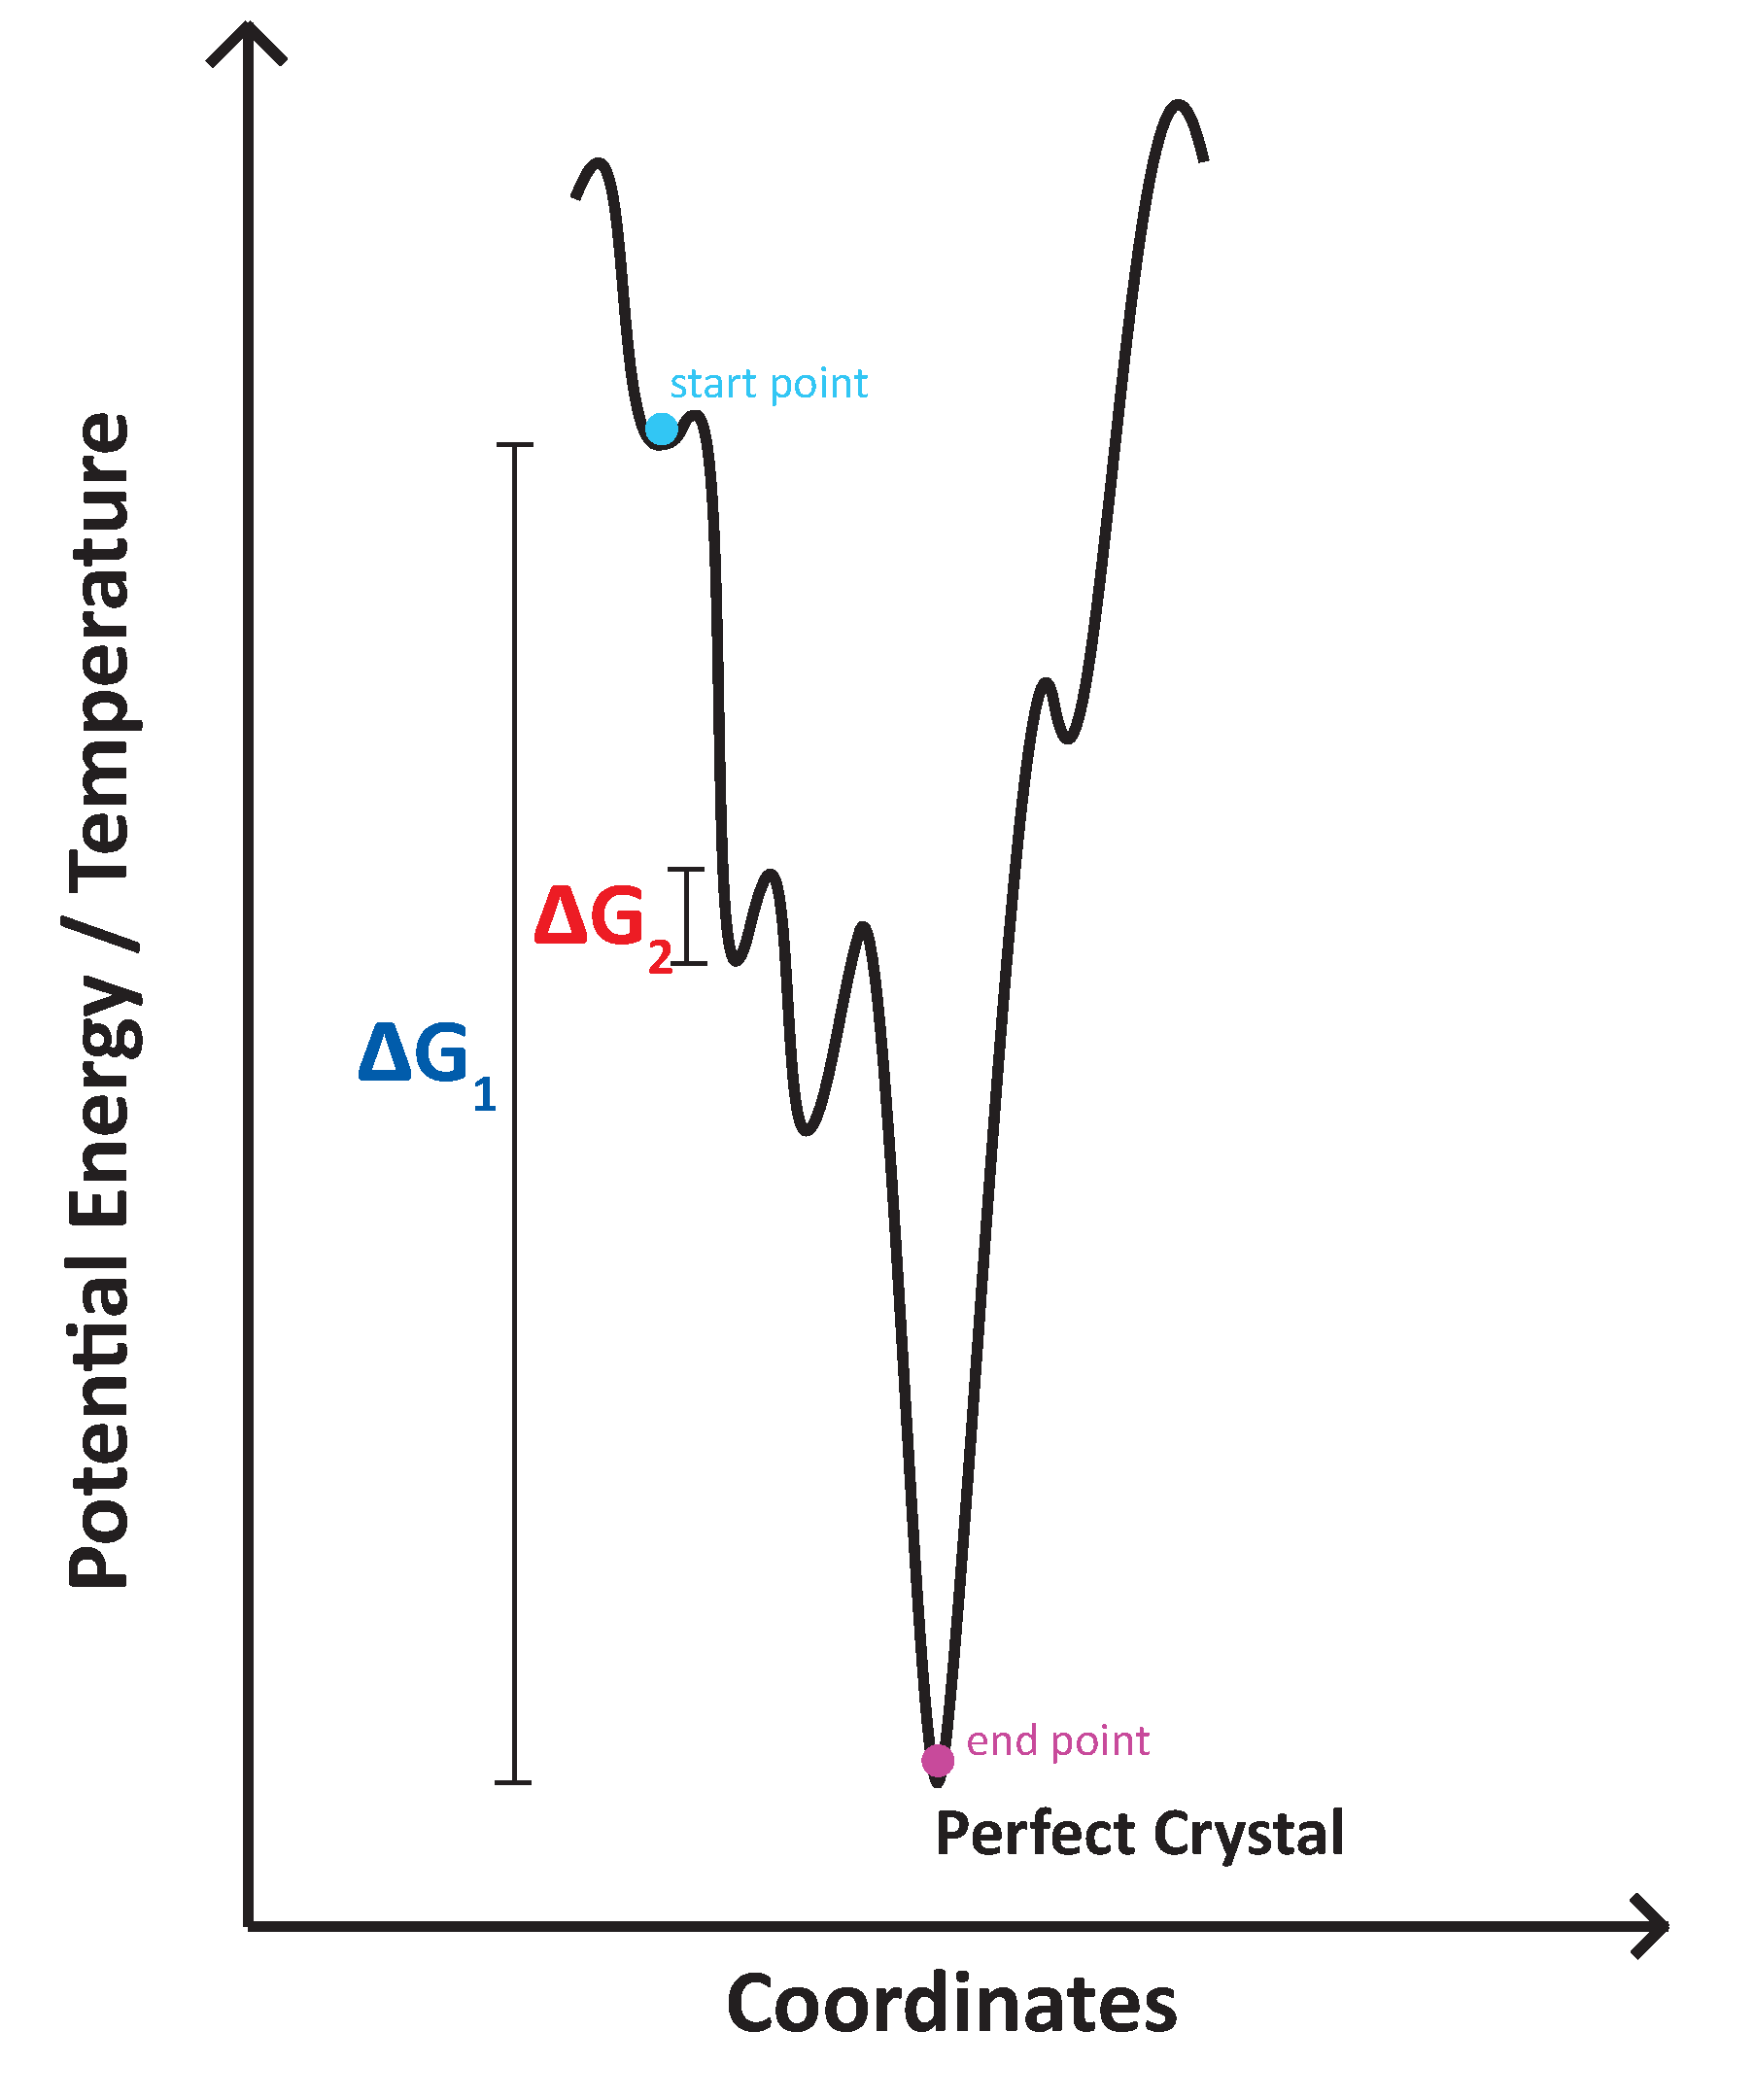
\includegraphics[width=.5\textwidth]{./Figures/Nucleation/nucleation_landscape.pdf}
	\caption{This figure shows a schematic drawing of the energy differences calculated from the energy landscape.  The colors for $\Delta G$ 1 and 2 correspond to the colors in Figure \ref{barriers}.  $\Delta G_1$ is the energy difference between the perfect crystal state and a given energy landscape basin.  $\Delta G_2$ is the energy difference of between the neighboring saddle point and the energy basin.  The schematic drawing also shows the starting point and end point of a theoretical metadynamics simulation along the energy landscape.}
	\label{barriers_origin}
\end{figure}

Figure \ref{barriers_origin} shows how the energy barrier for nucleation and crystal growth can be extracted from the energy landscape.  The schematic drawing that the starting point is from a high energy basin, and the end point is the perfect crystal lowest energy basin.  Between the two basins is a series of energy barriers and energy basins that are sampled along the way.  The figure shows the two energy differences involved in the simulation.  The first energy difference is the neighboring energy barrier separating two energy basins.  As explained previously, this is the energy barrier for dynamical behavior.  In this study, we assume that this barrier is the barrier for crystal growth.  This is justified by the idea that as an energy barrier is crossed the subsequent basin is of lower energy and generally greater structure.  Therefore, this barrier is the barrier for the addition of atoms to the new phase.  Similarly, since these barriers generally represent dynamics, such as atomic diffusion, and crystal growth is generally believed to be dictated by the diffusion of atoms to the crystal site, we logically connected these energy barriers to the crystal growth process.  This barrier is colored red to correspond to the color in the subsequent figures.  

The second energy difference in the system is the difference in system energy between the energy basins and the lowest energy basin energy.  This energy difference labeled $\Delta G_1$, is the difference between the perfect crystal state and the two phase (liquid and solid) or the single phase (liquid) state.  We have equated this energy difference to the energy required for formation.  This connection comes from the idea that to introduce the new phase comes with a certain energy cost, and this energy difference is the cost of the new phase induction.  This is similar to the CNT idea of calculating the nucleation free energy barrier.  However, rather than calculate the energy difference as a function of cluster radius as CNT does, we have calculated this energy difference without any macroscopic properties or \textit{a priori} assumptions about cluster shape.  This energy difference is also colored to correspond to subsequent figures.

\begin{figure}[h]
	\centering
	\includegraphics[width = .45\textwidth]{./Figures/Nucleation/high_density/TemperatureMapping.pdf}
	\hspace{.03\textwidth}
	\includegraphics[width = .45\textwidth]{./Figures/Nucleation/low_density/TemperatureMapping.pdf}
	\caption{Temperature mapping for the two simulations.  The left figure is for the high density system and the left figure is for the low density system. Red open circles are the data points from MD simulations, and the blue line is the data fit from the equation listed in the figure.}
	\label{temperature}
\end{figure}

As discussed in the previous chapter, in order to obtain useful information from the energy landscape is to be able to project the analysis into temperature.  Figure \ref{temperature} shows the two temperature mappings for the two system densities.  Before applying these to the energy landscape, the two figures show very distinct features.  First, the range over which the transition of high energy to low energy states occurs is dramatically different for the two systems.  The low density system has a transition over roughly ~30 K and the high density occurs over roughly ~10 K.  Further, for the high density case, there is a larger variance in values below the transition temperature than in the low density case.  Presumably this is due to the rougher energy landscape of the high density case, which means that it is easier for the system to be trapped in a metastable state than in the low density  case.  It is important to note that the data fit for the high density case is biased to pass through the lowest energy state rather than through points that reduce the residual, because if the fit does not cover the full range of energy values of the energy landscape then the mapping of the landscape to temperature fails.  The transition temperature for each density will be discussed later.

\begin{figure}[h]
	\centering
	\includegraphics[width = .45\textwidth]{./Figures/Nucleation/high_density/activation_energies.pdf}
	\hspace{.03\textwidth}
	\includegraphics[width = .45\textwidth]{./Figures/Nucleation/low_density/activation_energies.pdf}
	\caption{The activation barriers calculated from each simulation versus temperature.  The left figure is for the high density system and the right figure is for the low density system.  The figures show the activation barrier for crystal growth in red circles, the formation of a nucleation site in blue squares, and the total (sum of the two) in green triangles.  }
	\label{barriers}
\end{figure}

Extracting the energy differences from the sampled energy landscape and mapping to temperature are shown in Figure \ref{barriers}.  Figure \ref{barriers} shows the formation energy in blue squares, the growth energy in red circles and the total in green triangles.  There are many important features displayed in these figures.  First the two figures show a clear non-monotonic nature to the total energy difference in the system.  Second, the figure shows that different energies dominate at different temperature regimes.  At low sub cooling, the formation energy is high and thus nucleation sites are rarely formed.  At high sub cooling the formation energy is low and thus nucleation can occur more readily.  On the other hand, at low sub cooling the growth energy is low, because dynamics are quicker in this regime.  At high sub cooling the growth energy is high, because the dynamics are much slower as the glass transition temperature is reached.  Clearly from this figure, the low subcooling regime is dominated by formation energy differences, and at high subcoolings the regime is dominated by growth energy differences.  The high density figure did not show increase in total energy at lower temperatures most likely from lack of sampling a lower temperature regime, we believe if the data set was extended to lower temperatures the total energy would turn upwards again like in the low density case.

\section{Nucleation Rate and Interpolation to Time}
At this point, we employ classical nucleation theory.  While classical nucleation theory has been shown to inaccurately predict the free energy barrier involved in nucleation and crystal growth, the use of free energy differences to calculate the rates is still considered a correct methodology.  Classical nucleation makes the claim that the nucleation rate is proportional to the energy barrier by the following equation
\begin{equation}
\dot{N} \propto \exp\left( -\frac{\Delta G_{formation}}{k_BT}\right)
\end{equation}
where $\dot{N}$ is the nucleation rate.  We believe that with the metadynamics method employed in this study we have more accurately calculated the free energy barrier needed to calculate the nucleation rate.  Similarly, the crystal growth rate is calculated by
\begin{equation}
\dot{I} \propto \exp\left( -\frac{\Delta G_{growth}}{k_BT}\right)
\end{equation}
By using these equations, the trend of the nucleation, crystal growth, and overall crystallization rate is plotted in Figure \ref{rates}.  The overall rate is equal to the product of the nucleation rate and the crystal growth rate.

\begin{figure}[h]
	\centering
	\includegraphics[width = .45\textwidth]{./Figures/Nucleation/high_density/trend.pdf}
	\hspace{.03\textwidth}
	\includegraphics[width = .45\textwidth]{./Figures/Nucleation/low_density/trend.pdf}
	\caption{Exponential of the activation barriers versus temperature.  The left figure is for the high density system, and the right figure is for the low density system.  The red circles is for the growth of a nucleation site, the blue squares are for the formation of a nucleations site, and the green triangles are the sum of the two.  The pre-factor $J_o$ is the factor to relate these quantities to the crystallization rate of the system.  }
	\label{rates}
\end{figure}

Figure \ref{rates} shows the temperature dependence of the nucleation, crystal growth, and crystallization rate as determined by the energy barriers calculated from the metadynamics simulations.  From these figures, we can see that at low sub cooling the phase transition is limited by the formation rate and the growth rate is high.  Similarly, at high sub cooling the transition is limited by the growth rate due to slow dynamics of the system.  Further, we see that at a particular temperature roughly 301 K and 45 K for the high density and low density systems respectively, the overall rate has a maximum, and there is a transition from growth dominated to formation dominated.  As discussed in the introduction, this is expected.  

\begin{figure}[h]
	\centering
	\includegraphics[width=.45\textwidth]{./Figures/Nucleation/LJ_phase_density.png}
%	\hspace{.03\textwidth}
%	\includegraphics[width=.45\textwidth]{./Figures/Nucleation/Lj_transition_temperature.png}
	\caption[Coexistence curve for Lennard-Jones argon system as a function of normalized density and normalized temperature in Lennard-Jones units. F represents the fluid regime, G is for gaseous and L is for liquid, and S is for solid or crystalline.  The dashed horizontal line at around T = .7 Lennard Jones units is the coexistence line for freezing from a liquid to a solid.  This is also 84 K.]{Coexistence curve for Lennard-Jones argon system as a function of normalized density and normalized temperature in Lennard-Jones units \cite{Hansen1969}. F represents the fluid regime, G is for gaseous and L is for liquid, and S is for solid or crystalline.  The dashed horizontal line at around T = .7 Lennard Jones units is the coexistence line for freezing from a liquid to a solid.  This is also 84 K. \cite{Hansen1969}}
	\label{LJ_phase_density}
\end{figure}

As a sanity check that these temperatures in Figure \ref{rates} are physical, we can compare the results with a coexistence curve for Lennard-Jones shown in Figure \ref{LJ_phase_density} \cite{Hansen1969}.  Figure \ref{LJ_phase_density} shows the density versus temperature phase diagram \cite{Hansen1969}.  From this figure, we can see that for the low density case, of about 0.728 in reduced units, has a freezing temperature of 0.7 in reduced units, or 84 K.  This means that we are predicted that for homogeneous nucleation to occur, the system must be around 10 K sub cooled.  Further, at 40 K sub cooled, we see a maximum in transition rate.  The reported glass transition temperature for this density is roughly around ~24 K, thus for us to predict the rates to decrease near 30 K is reasonable.  Similarly, from Figure \ref{LJ_phase_density}, we can approximate the melting temperature for the high density system, of a about 1.25 in reduced units, to be near 360 K by extrapolation of the data in Figure \ref{LJ_phase_density}.  Further, we predict from our temperature mapping that a transition to landscape dominated to be near 310 K, or 50 K subcooling.  

One of the largest advantages to metadynamics, compared to Monte Carlo, is that the simulation can provide temporal information, which is generally macroscopically long compared to molecular dynamics.  It provides information about dynamics through the energy barriers.  However the simulation itself typically can not be analyzed as a function of time, because the simulation is a function of penalty number.  However, from the original energy landscape framework, the dynamical behavior is described as the transition from one basin to another.  Thus, from the metadynamics simulation, we consider that the simulation is a series of basin hopping.  Thus, if we know the average time for the transition from one basin to another, we can interpolate the metadynamics simulation to time \cite{Cavagna2009}.  We can predict this average time as the relaxation time for the system to relax from one basin to another.  The relaxation time for basin transitions is commonly displayed as
\begin{equation}
\tau = \tau_M\exp\left( \frac{E_A}{k_BT}\right)
\end{equation}
where $\tau$ is the relaxation time, $\tau_M$ is the Maxwellian relaxation time, $E_A$ is the activation energy for the transition \cite{Dexter2009}.  Thus, since we know the activation energy separating the energy basins sampled in the simulation, and the Maxwellian relaxation time can be calculated from an Arrhenius law
\begin{equation}
	\tau_M = \frac{\eta}{G_\infty}
\end{equation}
where $\eta$ is the viscosity and $G_\infty$ is the shear modulus \cite{Dexter2009}. The Maxwellian relaxation time is reported on the order of hundreds of femtoseconds \cite{Dexter2009}.  There is variability for the density, but for now, order is sufficient \cite{Dexter2009}.  By assuming the time to cross an energy barrier and transition from one basin to another, the energy landscape can be plotted as a function of time.

\begin{figure}[h]
	\centering
	\includegraphics[width=.45\textwidth]{./Figures/Nucleation/high_density/time.pdf}
	\caption{The energy landscape extrapolated from a function of penalty number to a function of time.}
	\label{time}
\end{figure}

Figure \ref{time} shows the energy landscape for the high density simulation as a function of time in picoseconds.  As a sanity check that this is the correct approach for time extrapolation, a research group used MD simulations of Lennard Jones argon with identical box size and number of atoms as we used \cite{Park2004}.  The group, knowing MD cannot capture nucleation, induced the nucleation process with a field \cite{Park2004}.  By inducing the nucleation event they studied the system over time \cite{Park2004}.  They used a time step of 5 fs and determined the system took 80,000 time steps to achieve a crystal state \cite{Park2004}.  The group also studied the energy landscape during the simulation and noticed a similar pattern of plateaus in the potential energy representing different structures in the system \cite{Park2004}.  By comparing this groups reported 400 ps time for crystallization, and Figure \ref{time} which shows we approximate a time of around 310 ps, we conclude that using the Maxwellian relaxation time and Arrhenius trend to extend our simulation into time is well founded.  We believe these two times are in good agreement given the relative error in relaxation time used, the MD simulation, and our own simulation.


\chapter{Energy Landscapes of a Glass Former and Crystal Former}
\label{compare landscapes}
In this chapter, we extend the metadynamics simulation to a binary Lennard-Jones liquid.  The Kob-Andersen model is a known glass former.  By applying metadynamics to both a fragile glass former (Kob Andersen model) and a poor glass former (monoatomic Lennard-Jones), we can get a more thorough understanding of the energy landscape.  Herein, we define a good glass former (the fragile glass forming system) as a system that is likely to form a glassy state without extreme conditions applied to frustrate the crystal state.  We define a poor glass former, or a good crystal former (the monoatomic Lennard-Jones system), as a system that is likely to equilibrate to the crystal state, and therefore not likely to form a glassy system unless extreme conditions are applied to frustrate the crystal state.  These definitions are to help the reader.

\section{Theory and Background}
As discussed in Chapter \ref{metadynamics}, the energy landscape has been a highly successful picture for detailing the behavior of materials both in and out of equilibrium, the relaxation of metastable materials, and the difference between alpha and beta relaxations \cite{Royall2015}.  However, as a theoretical concept, the energy landscape is difficult to prove with any experimental evidence.  There is no physical or experimental method that can directly sample the energy landscape.  Further, due to the high dimensionality of the energy landscape, detailing the full energy landscape is difficult from simulations as well.  Thus, despite a large amount of recent work using the energy landscape to explain physical phenomena, no direct evidence exists to proof what we believe the landscape to look like.  

As previously discussed, it is believed that the energy basin for the crystal state is narrow and extremely deep (generally the deepest basin on the landscape, depending on the number of crystal polymorphs \cite{De2014}).  Similarly, it is often theorized that metastable basins are deep while not as deep as the crystal state, and often described as broad \cite{De2014}.  The glassy basins are described as rich with small and large energy minimums separating the multitude of energy minimums within a local region of the landscape \cite{De2014}.  However, since the landscape has generally remained a theoretical framework, the distinction between landscapes of glass formers and crystal formers has remained merely theoretical.  

We have already shown the potential of metadynamics to sample a trajectory along the energy landscape.  Thus, by employing the metadynamics method we have implemented, we can directly sample the energy landscape of a good glass former and a good crystal former and determine the actual difference between the two landscapes.  We have already shown the density effects on the landscape.  Now, we show unique features between a good crystal and good glass former.

\section{Results}
\label{kob_andersen}
Metadynamics was applied to two distinctly different systems, a monoatomic Lennard-Jones argon and a binary Lennard-Jones system.  The monoatomic Lennard-Jones system is identical to the system used in the previous chapter for studying nucleation and crystal growth.  The system was composed of 864 Lennard-Jones argon atoms, with parameters $\sigma = .340$, and $\epsilon = .9977$.  The metadynamics parameters used were penalty height of 1 kJ/mol, a height squared of .1 nm$^2$, a maximum number of penalties of 20,000, a initial minimization step of .0001 nm, and the structural restraints were disabled.  The binary Lennard-Jones system was composed of 178 atoms of type A and 45 atoms of type B, or roughly a ratio of 80:20, the Lennard-Jones parameters were $\sigma_{AA} = .340$, $\sigma_{BB} = .299$, $\sigma_{AB} = .272$, $\epsilon_{AA} = .9977$, $\epsilon_{BB} = .4989$, $\sigma_{AB} = 1.4966$ \cite{PhysRevE.51.4626}.  This is the well known Kob-Andersen system \cite{PhysRevE.51.4626}, and is a well known glass forming system.  The metadynamics simulation parameters were a penalty height of 1 kJ/mol, penalty width squared of .1 nm$^2$, a maximum number of penalties of 2,000,000, an initial minimization step of.001.  The monoatomic system was simulated for 2 hours with 12 processors, and the binary Lennard-Jones system was simulated for 20 hours with 12 processors.  The difference is because the nucleation and crystallization process completes quickly on the monoatomic system.  The potential energy sampled by the two simulations are shown in Figure \ref{compare_landscape}.

\begin{figure}[h]
	\centering
	\includegraphics[width=.45\textwidth]{./Figures/Landscape/glassy_landscape.pdf}
	\hspace{.01\textwidth}
	\includegraphics[width=.45\textwidth]{./Figures/Landscape/crystal_landscape.pdf}
	\caption{Potential Energy versus penalty number for two simulations.  The left figure shows the potential energy sampled for a binary Lennard-Jones system known for being a fragile glass former.  The right figure shows the potential energy landscape sampled for a monoatomic Lennard-Jones system known for being a poor glass former.}
	\label{compare_landscape}
\end{figure}

Figure \ref{compare_landscape} shows the energy landscapes sampled by the two simulations.  The left figure shows the binary Lennard-Jones system and the right one shows the monoatomic Lennard-Jones.  The first major aspect to notice is the difference in scales.  The monoatomic system has only 5000 penalties applied whereas the binary system has nearly 20,000 penalties applied.  This is due to the fact that the monoatomic system had a finite duration, added more penalties once it was in the deep crystal minimum only resulted in vibrations of the crystal lattice, thus applying more penalties resulted in extraneous information.  This helps prove that the crystal state minimum is deep and narrow, because even after adding many more penalties the system never began to re-climb out of the minimum, we never saw the system become disordered again.  Conversely, the binary system required the application of as many penalties as possible in order to get thorough sampling of the entire landscape.  We needed good statistics of the landscape for a separate analysis of this system.  When viewing the real space movie of the binary system and when looking at the bond order parameter, the system never showed signs of order.  

The next major observation to make about the two landscapes is that for the monoatomic system, the potential energy generally only decrease after overcoming a barrier.  This is indicative of a funnel like landscape.  The landscape is rather simple and the gradient of the landscape ubiquitously points downwards towards the crystal state.  Comparatively, the binary system landscape has neighboring basins that are greater than and less than the previous basin.  Further, with more analysis, the binary system can be shown to be rich in both small local energy barriers and also large energy barriers separating distance broad basins.  These two figures lend great support to the theorized differences between the landscapes of poor glass formers and fragile glass formers.

\begin{figure}[h]
	\centering
	\includegraphics[width=.45\textwidth]{./Figures/Landscape/glassy_time.pdf}
	\hspace{.01\textwidth}
	\includegraphics[width=.45\textwidth]{./Figures/Landscape/crystal_time.pdf}
	\caption{Potential Energy versus penalty number for two simulations.  The left figure shows the potential energy sampled for a binary Lennard-Jones system known for being a fragile glass former.  The right figure shows the potential energy landscape sampled for a monoatomic Lennard-Jones system known for being a poor glass former.}
	\label{compare_time}
\end{figure}

Like in the case of the nucleation study, the landscape for the binary system can be extended to the time scale rather than as a function of penalty number.  Figure \ref{compare_time} shows the energy landscape sampled as a function time.  The time scale has not been adjusted to real time units, rather it is still in terms of the Maxwellian relaxation time for the system.  As the figure shows, the binary system has a time scale orders of magnitudes larger than the monoatomic system.  Further we can see that the monoatomic system as previously shown samples gradually along the landscape in time.  Whereas, the binary system has very clear long time periods in which the system is stuck in a deep metastable state.  Similarly, the binary system when overcoming a large barrier spends very little time in the high energy state and quickly becomes stuck in a metastable basin again.  This shows that glassy dynamics are very explainable by the energy landscape.  Small time scale relaxations are related to the small energy basins within a deep metastable state, and long time relaxations are dominated by extremely large energy barriers separating deep energy basins.  

By showing the different aspects of the energy landscape for good glass formers, good crystal formers, and different densities of a good crystal former, we can use metadynamics to sample the energy landscape of a system and make predictions about the systems behavior.  The landscape can show if the system is a good glass or crystal former.  The landscape can predict rates invovled in the system, and can provide energy barriers of different timescales.

\chapter{Conclusions and Future Work}
\section{Conclusions}
In this thesis, we applied the recently successful energy landscape framework and metadynamics method to study nucleation and crystal growth, and compared the energy landscapes of a fragile glass former and a good crystal former to verify the energy landscape framework with the metadynamics method.  Traditional molecular dynamics is hindered by temporal limitations and Monte Carlo lacks dynamical information prohibiting these two methods from capturing the nucleation and crystal growth process fully.  As a response, we successfully implemented metadynamics into the open source package GROMACS with full OpenMP parallelization.  Metadynamics simulations allowed us to calculate the free energy barrier as a function of temperature involved in the nucleation and crystal growth process.  Unlike many other methods to compute this free energy barrier, metadynamics requires no \textit{a priori} assumptions for the calculation of the free energy barrier.  Thus, we believe that the use of metadynamics is more accurate for the calculation of this energy barrier and non-monotonic nucleation rate. 

Herein, we applied the metadynamics method to a model liquid monotonic argon system, and sampled the energy landscape.  From the potential energy landscape, we were able to determine the energy barriers involved in the nucleation and crystal growth process.  We determined that there are two unique energy barriers involved in the process, and each one dominates in a different regime.  At high subcoolings, the crystallization process is diffusion limited, and the crystal growth energy barrier dominates the crystallization process.  At low subcoolings, the crystallization is kinetically limited, and the formation of nucleation sites limits the crystallization process.  We find a non-monotonic temperature dependence of the overall crystallization energy barrier and rate.  Further, we apply metadynamics to a binary Lennard-Jones system, which is a known good glass former.  By comparing the monotonic Lennard-Jones system to the binary Lennard-Jones system, we are able to see the stark difference between the energy landscapes during crystallization and during glassy dynamics.

\section{Future Work}
Thus far, we have had great success with the metadynamics method.  The method was successfully built into the open source package GROMACS, with the addition of dynamic minimization step sizing and OpenMP parallelization.  Also, the method was successfully used to study nucleation in a LJ system and used to computationally confirm the differences in the energy landscape between good glass formers and good crystal formers.  However, a great deal of future work still exists.  The three categories of future work can be summarized into further application of the method to new systems, further analysis of the simulations, and development of enhanced metadynamics methods.

\begin{itemize}
	\item \textbf{Applications/systems}  
	In this thesis, we demonstrated two important applications of the metadynamics method.  We applied the metadynamics method to study crystallization in a monoatomic Lennard-Jones system, and also applied the method to study a fragile glass forming binary Lennard-Jones for comparison to the monoatomic counter part.  Lennard-Jones is a great starting potential because it is very well studied, simple to apply, and simple to understand. In particular, Lennard-Jones is known to exhibit an FCC crystal structure.  However, we wish to extend our work by applying the metadynamics method developed herein to more complex potentials and more application relevant materials (Lennard-Jones is not real-world common).  
	
	There are several systems we wish to extend this analysis to.  First, we wish to study ST2 water with this method.  We have already begun simulations of this system (both MD simulations and MTD simulations).  The full details of our preliminary results of the model is contained in Appendix \ref{ST2}.  The ST2 model and water in general is known to have several crystal polymorphs, exhibit supercooled behavior, and is critical in an application sense \cite{Haji-Akbari2015}.  We hope the metadynamics method may elucidate why one polymorph is dominate at different points in the phase diagram.  Another potential application is to apply metadynamics to a thin film system.  This would allow us to study surface behavior of a system.  We also wish to apply the method to protein systems in order to study the folding-unfolding process which is macroscopically magnitudes longer than MD can capture.  Lastly, the possibility to study metallic systems is available if we extend the method to LAMMPS \cite{LAMMPS}, another open source MD package known for studying metallic systems.
	
	Another study we wish to perform is the study of the landscape and the effect on fragility of glass formers.  In this thesis, we already provided insight to the differences between fragile glass formers and poor glass formers.  We wish to extend this to strong glass formers and fragile glass formers of varying degree.  Then, we can find a connection between the landscape statistics, roughness, and other landscape quantities to the glass formers fragility.  This could offer insight or at least provide a theoretical explanation for the difference in glass formers behavior, and potentially offer a predictive method for estimating new glass formers fragility.
	
	Lastly, we wish to apply metadynamics to other known macroscopically long timescale events, such as material aging and  degradation.  Both of these events can occur on orders of magnitude longer timescales than accessible to molecular dynamics simulations.  By using metadynamics, we can observe the material aging and degradation process from an atomic scale.  
	
	\item \textbf{Further Analysis}
	
	%% determine J_o
	Metadynamics simulations, like MD and MC simulations, requires a great deal of analysis to extract useful information from the simulation.  While this report various analysis of a MTD simulation, there is still a great deal of information hidden in the simulation that requires extraction.  First, we have successfully computed the potentially energy barriers involved in the nucleation process and estimated the time scale involved in the process.  However, in order to fully benchmark our results to experiments we need to compare to known nucleation and crystallization rates, which requires us developing a method to compute $J_o$, the scaling factor for the nucleation rates we calculated.  We wish to estimate this value from the simulation and compare to experiments, rather than extract the value from experiments.
	
	%% determine frequency distributions to compare to REMA
	Recent work by Cai et. al. showed that they could extract the activation barriers and frequencies from simulations and experiments via a transform of the dynamic structure factor \cite{CaiREMA}.  We have thus far been able produce comparable activation barrier distributions as a function temperature for the same binary Lennard-Jones system \cite{CaiRMA}.  We wish to extend our analysis to be able to also reproduce their frequency distribution results.  Metadynamics is capable of providing the activation barrier information by sampling the energy landscape, however, our method does not contain true dynamics making calculation of the frequencies difficult at this moment.  We hope to calculate the frequencies by in parallel with the Metadynamics simulations run MD simulations with small energies to calculate the frequency distributions.
	
	%% compare to insitu diffraction patterns
	Experimental studies of nucleation is widely known.  However, recent work with an electro static levator and X-ray/Neutron scattering diffraction experiments have given hope that experimental investigation of the structural changes during nucleation maybe possible.  The electro static levator suppresses the heterogeneous nucleation in a sample and scattering experiments provide a probe to measure atomic structure.  As long as the flux is sufficiently high, time resolved inspection of homogeneous nucleation might be possible and would allow direct comparison to our simulations.
	
	\item \textbf{Enhanced Methods}
	
	While the metadynamics method has already shown great success, it can still be greatly improved upon.  The strength of the metadynamics method is dependent on the number of minimums and saddles points sampled, which is dependent on the number of penalties applied during the simulation.  As shown previously in this report, as more penalties are applied the time for the system to converge to a new minimum linearly increases due to the increased computational cost of computing the forces in the system.  Therefore, in order to study large systems such as proteins, we need to sample a large amount of barriers in an efficient amount of time.  As a result, we are pursuing a few new methods for improving on the sampling methods used in this report.  
	
	We have already tried a few enhanced methods, which are shown in depth in Appendix \ref{enhanced methods}.  Briefly, we attempted two methods of variable reduction.  One way to increase the speed of the metadynamics is to decrease the number of reaction coordinates.  However, determining which reaction coordinates are relevant and which are extraneous is a nontrivial task.  We developed two methods, bond order restrained metadynamics and bond order restrained with dynamic unfreezing metadynamics, to determine which variables are extraneous.  The two methods used the bond order parameter to determine which atoms were considered structured and would freeze these atoms, thus reducing the number of forces computed on each iteration.  The dynamic freezing option allowed atoms to become unfrozen if the bond order parameter fell below a threshold value.  While these methods increased the number of penalties applied to the system, the method also removed the variables necessary for crystal growth to occur.  The results of these methods are summarized in Appendix \ref{enhanced methods}  
	
	Another method we attempted for enhanced sampling was coined ``steepest ascent,'' which inverts Newton's steepest descent method.  The goal of the method was to use steepest descent for energy minimization to converge on a local minimum, then to use steepest ascent to converge on a local maximum or saddle point.  However, the method's down side is it is highly unstable and often converges to global maximum (infinite potential energy) rather than converging to the low energy saddle points.  We further attempted introducing methods to prevent the method from converging on infinite energy maximum, but saw little success yet. The results of this method are fully explained in Appendix \ref{enhanced methods}.  
	
	Even though these methods have not produced concrete results as of yet, we plan to continue developing these methods as the foundation for a more robust and efficient metadynamics method.  We believe with further work and development of the ideas behind these methods then when they come to full fruition, the methods will produce viable results in a far more effective and efficient manner than the metadynamics method used in this report.
\end{itemize}

\appendix
\chapter{Implementation of Metadynamics into GROMACS}
\label{code}
%% Make schematic drawing of the flow of the code into gromacs, make a flow chart to show how the implementation was made (this will help emphasize the difficulty it took to place into the program)
GROMACS is an open-source molecular dynamics package primarily designed for the study of soft, organic systems such as water and proteins.  The code is developed majoritively  in C, at least the version we utilized is, but has extended some code to C++.  The package is considered extremely efficient because of its processor specific optimization and its implementation of OpenMP and MPI parallelization.  Unlike most reported metadynamics simulations, we integrated the metadynamics method fully into GROMACS rather than build a stand alone metadynamics simulation package.  GROMACS provided us a frame work such that we could focus on the metadynamics method and ignore other aspects such as developing force calculation from pair potentials, input/output, or generation of pair potentials.  

The implementation of metadynamics is fully functional in the sense that it does not effect any other aspect of the package.  GROMACS offers several simulation options including molecular dynamics, stochastic dynamics, Brownian dynamics, energy minimization, and normal mode analysis, thus to make our implementation fully compatible we added the simulation option metadynamics.  While fully compatible we need to do some house keeping to the code to conform to the GROMACS coding standard (naming convention, comment style, etc.) before we can request GROMACS to integrate the code into the next release.  The code also has been parallelized with OpenMP to allow multiple processor computation during a single simulation.  However, MPI parallelization has not been added yet which limits our simulations to only one compute node when submitting to compute clusters.

Implementation of metadynamics into GROMACS required the alteration of several source files in the package, however the main algorithm is contained to one file. The algorithm implemented into GROMACS has been visualized as a flow chart in Figure \ref{flowchart}, because inclusion of the code would be excessively long.  The flowchart shows the crucial calculations, loops, and decision tracks for implementing metadynamics.  The current version of the metadynamics implementation includes the adaptive minimization step size, optimized parallelization of loops, and our recent work on structurally restrained metadynamics, which is discussed further in Appendix \ref{enhanced methods}.
\begin{figure}
	\centering
	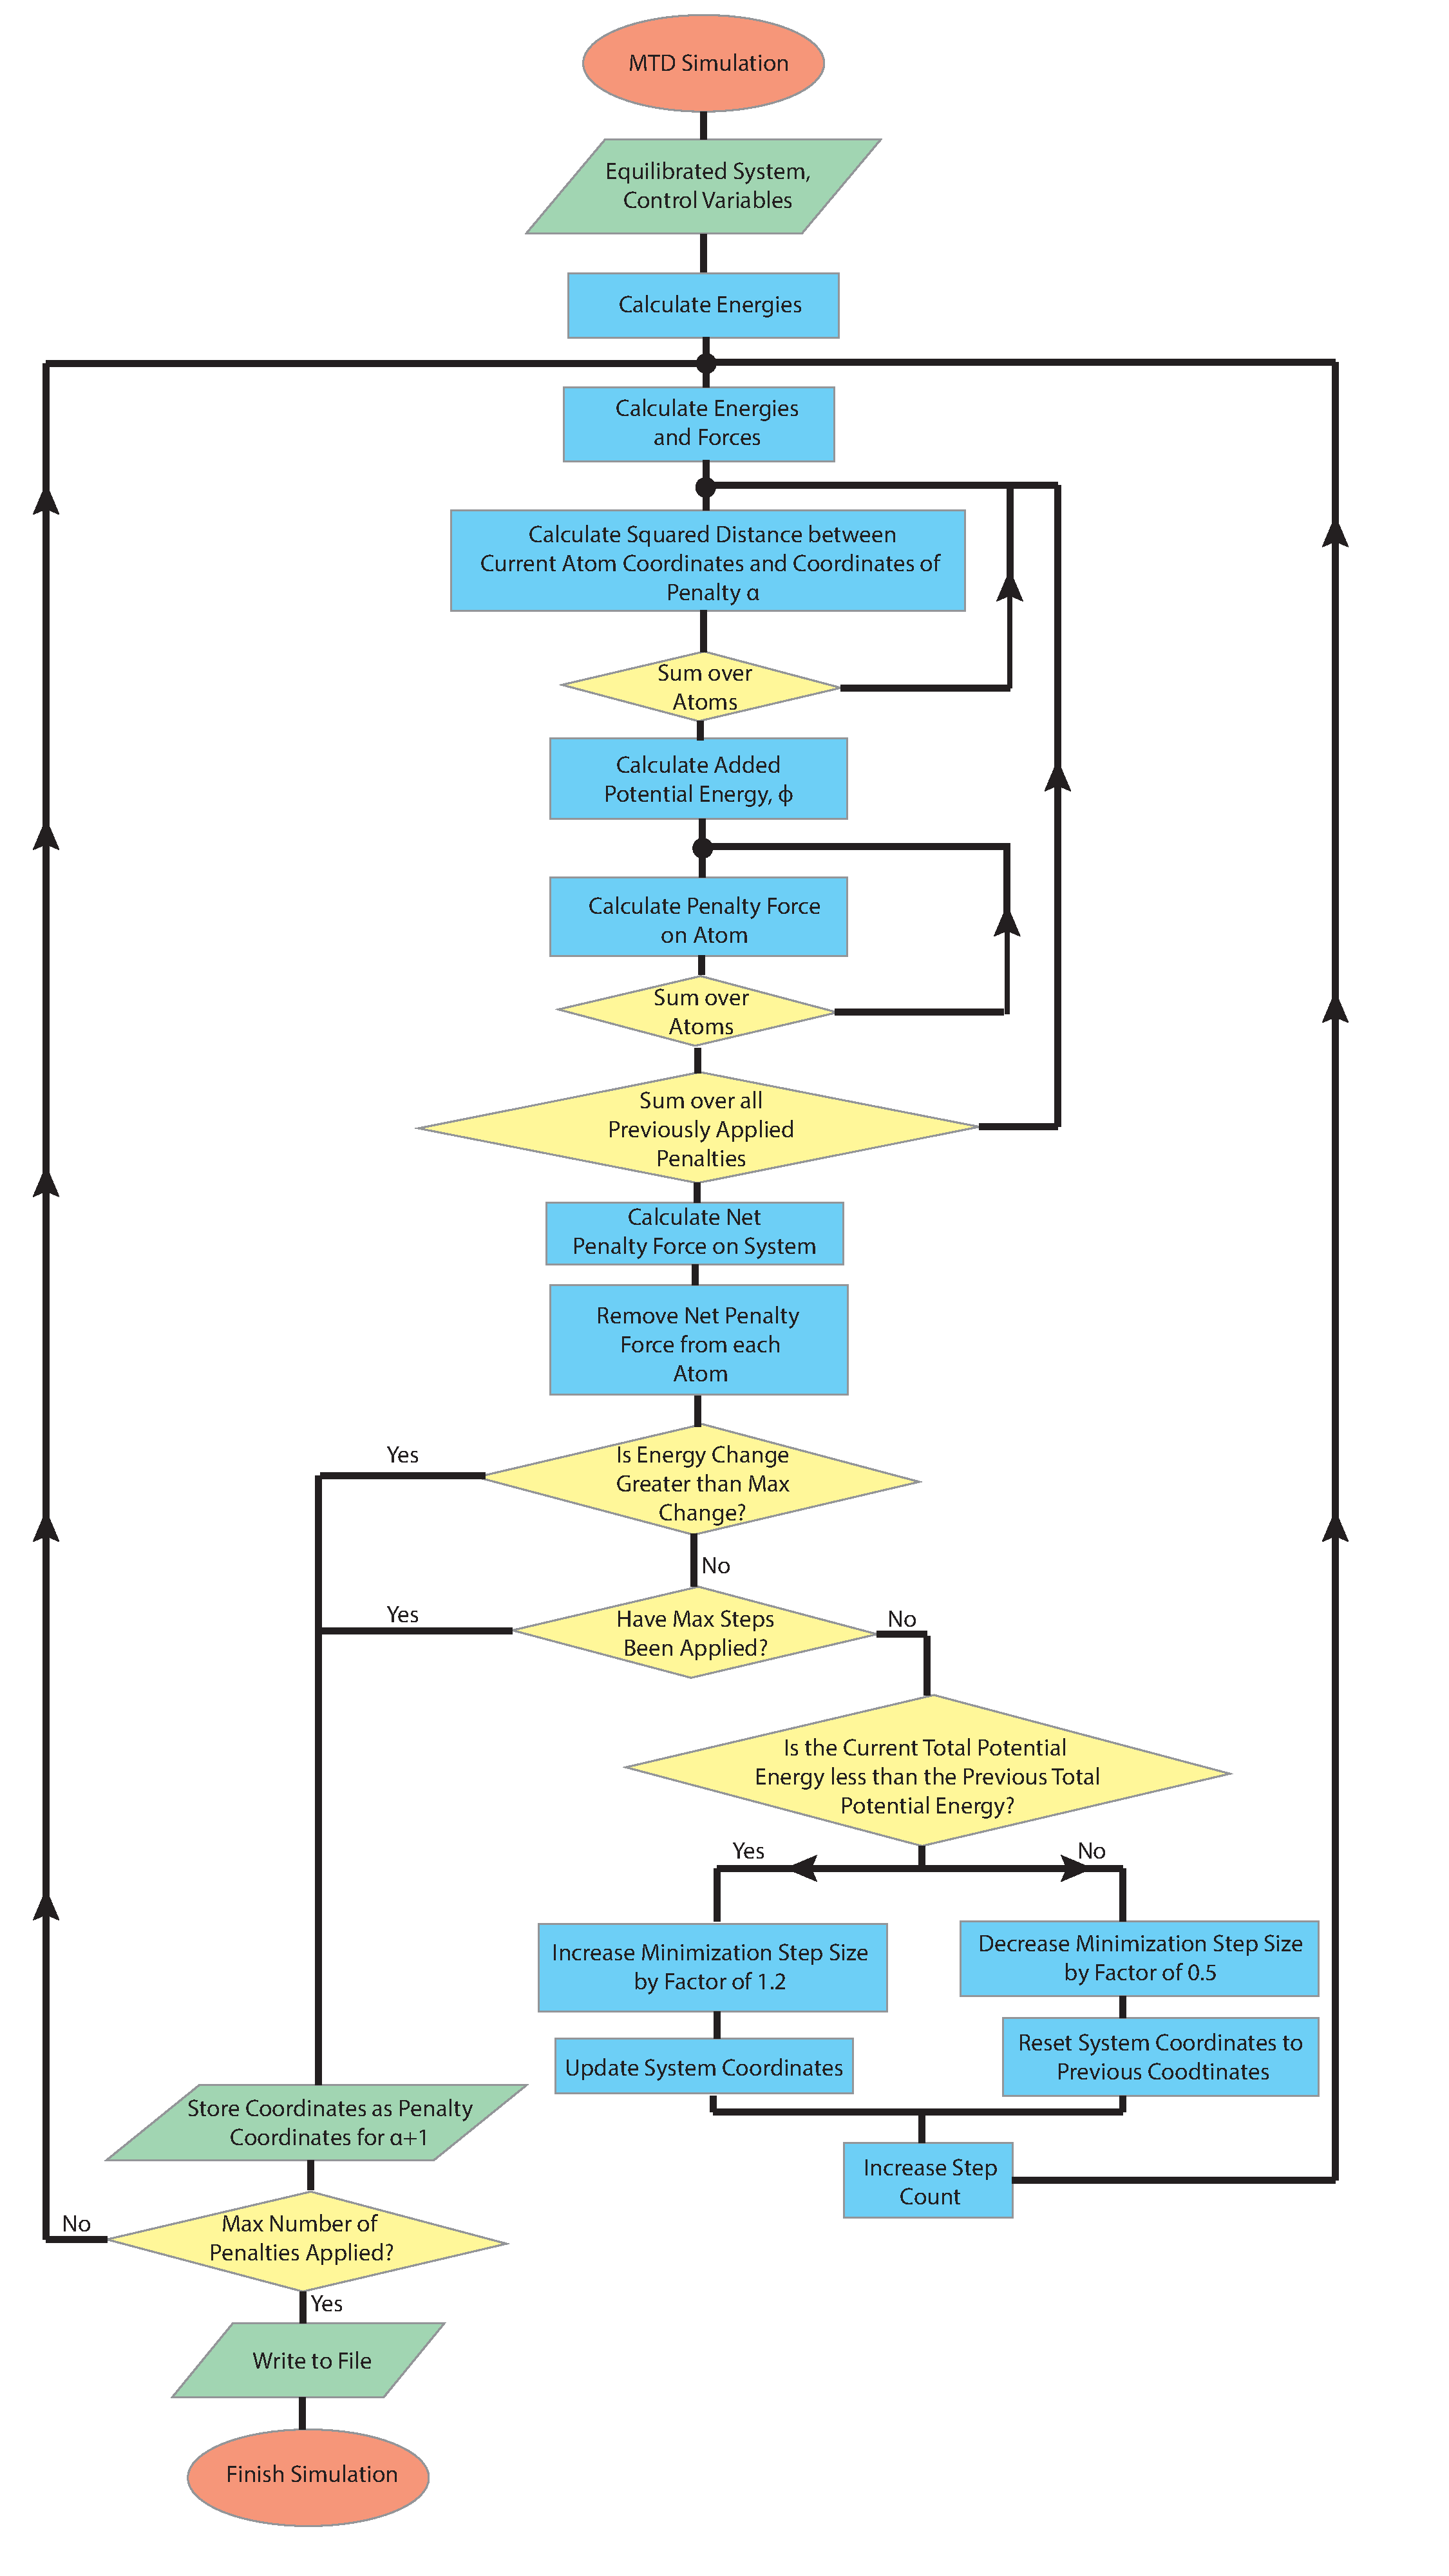
\includegraphics[height=.95\textheight]{./Figures/Appendix/MTD_flowchart.pdf}
	\caption{A schematic flow chart of the metadynamics code implemented into GROMACS.}
	\label{flowchart}
\end{figure}

\chapter{LiquidLib}
\label{LiquidLib}

With the recent increase in computational power, molecular dynamics (MD) simulations have emerged as a powerful tool for understanding and comparing to experimental results. MD and MC simulations have provided great insight across engineering and science fields alike, and have been applied to materials ranging from inorganic compounds like metals to biological systems such as protein and DNA. MD and MC simulations are especially imperative to the study of liquids and liquid-like systems, as they provide understanding to the structural and dynamical behavior of liquid systems in and out of equilibrium.  Similarly, researchers use MD and MC simulations to understand and interpret results measured by neutron scattering experiments.

These simulations result in trajectories that provide the positions, $\mathbf{r}_i(t_j)$, and the velocities, $\mathbf{v}_i(t_j)$, of the atoms, where the subscript $i$ refers to the $N$ different atoms in the system and the subscript j refers to the $M$ time steps. Simulations result in $6NM$ data values, which, to obtain meaningful results, need to be reduced to conceptually simpler, useful, and in many instances, measurable quantities. Reduction of these simulations to simpler and understandable quantities requires programs to perform these analyses.

Numerous open source and commercial packages exist to perform molecular dynamics and Monte Carlo simulations, but outside of a few simple quantities such as pair distribution function or mean squared displacement, these packages often do not offer the option to compute quantities needed to interpret the simulation or compare to experimental results for liquid systems. Thus, most researchers are forced to write in-house scripts and programs to compute the desired quantity, but these tend to only be useful to the respective researcher. On the other hand some codes can be obtained online to compute select quantities, but these are scattered, requiring users to seek out multiple packages, learn the code's implementation, and possible convert their trajectory to match the file type required by the package. As a result, a few attempts to create a comprehensive post-processing package for molecular dynamics simulations emerged, such as the open source software TRAVIS \cite{TRAVIS} or nMOLDYN \cite{nMOLDYN}. 

We introduce LiquidLib, an open-source and comprehensive package for post-processing of molecular dynamics and Monte Carlo simulations of liquids for comparison to neutron scattering experiments \cite{LiquidLib}.  LiquidLib was developed in the same spirit as TRAVIS \cite{TRAVIS} and nMOLDYN \cite{nMOLDYN} while greatly expanding on the capabilities of the packages.  LiquidLib extends the list of calculable quantities, the list of readable file types while also offering an easy method to add a file type if not already offered, and implements efficient parallelized C++ code to perform analysis in speeds unmatched by similar packages.  The goal of LiquidLib is to create a singular package to compute all desired quantities for studying liquid simulations. Further, LiquidLib is easily expandable to be able to read a simulation trajectory from any program. At the moment, LiquidLib can read trajectories from LAMMPS (.xyz, .xtc, .dump, .atom) \cite{LAMMPS}, GROMACS (.xtc, .trr, .gro) \cite{GROMACS}, and VASP (XDATCAR) \cite{VASP}, however we hope to expand on this list. The variety of trajectory data supported by LiquidLib allows users to run computations for systems with different length scales including atoms, molecules, colloids, coarse-grained models, and etc.  LiquidLib also contains a corresponding graphical interface to aid in the construction of input scripts and the analysis procedure.  LiquidLib's list of quantities currently includes the following, the pair distribution function, the static structure factor, the mean squared displacement, the non-Gaussian parameter, the four-point correlation, the velocity auto correlation, the self and coherent van Hove correlation, the self and coherent intermediate scattering functions, and the bond orientational order parameter.  LiquidLib offers the ability to weight quantities based on the neutron scattering lengths for multi-component systems, which allows the results to be comparable to neutron scattering experiments. 

While not extensively used, numerous studies into the behavior of colloids, liquids, and glasses with hyper-dimensionality have been performed in recent years \cite{Charbonneau2012, Charbonneau2013}. Similarly, we have also created an in-house package that simulates Lenard-Jones liquids in high dimensionality, which requires special care to analyze the trajectories in high dimensions. As a result, LiquidLib differs from other reduction packages in that the dimension of the simulation can be set to any positive integer and the quantities will be correctly calculated.  While LiquidLib was written for the context of liquids and liquid-like systems with comparison to neutron scattering experiments, the quantities calculable by LiquidLib are useful for non-liquids systems and comparison to analyses other than neutron scattering. Simple extension to compare with X-ray measured experiments corrected for atomic-form factors can be performed by unweighted computations whereby the scattering lengths are set to unity.

For the purpose of this project, LiquidLib was extended to incorporate the ability to read MTD trajectories from GROMACS.  Further, LiquidLib was extended to compute the bond orientational order parameter.  LiquidLib was developed as a side project to this project for the main purpose of MD simulations and extended to aid metadynamics simulations.  LiquidLib is developed and maintained by the Zhang Research Group, particularly at this time, by Zhikun Cai, Abhishek Jaiswal, and Nathan Walter \cite{LiquidLib}.

\chapter{Structurally Restrained Metadynamics and Steepest Ascent}
\label{enhanced methods}


\section{Objective and Theory}
The original metadynamics method presented in Chapter \ref{metadynamics} uses the all atoms spatial coordinates as the reaction coordinates in the metadynamics method.  This results in 3N degrees of freedom, 3 for the spatial coordinates and N for the number of atoms, which leads to super linear increases in computational costs for the metadynamics method.  As shown previously, the cost of applying a penalty function to the system also increases linearly as the number of penalties increases.  As a result, simulating large systems for sufficient penalties is difficult.  Often other applications of metadynamics choose to use a select few crucial reaction coordinates, such as bond angle in proteins or spatial coordinates of atoms of interest.  However, for a homogeneous predefining the reaction coordinates of interest is extremely difficult.  The goal is to reduce the number of coordinates from 3N used as reaction coordinates for metadynamics in order to more efficiently apply penalties.  This reduce the computational cost of each penalty and will lead to more efficient sampling of the landscape.  

\section{Bond Order Parameter Restrained Metadynamics}
There is no universal method for determining the coordinates of interest, however, methods can be developed based on the goal of the simulation.  For studying nucleation and crystal growth, the goal is to sample the energy landscape while driving the system from a high energy amorphous configuration to a low energy crystalline configuration.  We measure structure in the system with the sixth order bond orientational order parameter, as discussed in section \ref{bop_calculation}.  Thus, if we transform our picture of the energy landscape from spatial coordinates to bond orientational order parameter, the penalties are driving the system from low $\bar{q}_6$ values to high values.  With this understanding, we can justify reducing the variable space based on an atom's $\bar{q}_6$.  In algorithmic terms, the system begins uniformly with low $\bar{q}_6$ values.  Then as penalties are applied, some atoms may rearrange preferentially first, leading to regions of high $\bar{q}_6$ values.  If an atoms $\bar{q}_6$ value exceeds some threshold value, we can consider this atom to have already reached the global minimum of the landscape.  Therefore, we can now safely ignore the spatial coordinates of this atom as potential reaction coordinates, and no longer apply penalties to this atom.  The idea being that if nucleation truly begins from a seed and then grows throughout the system, then we can freeze the nucleation sites and allow the remaining atoms to grow onto the nucleation site.  As the cluster grows, we can freeze more atoms, thus as penalties are applied we can continue reducing the variable space until the global minimum is reached and the variable space becomes zero.  The benefit of this method is that it is finite in time, the simulation ends when all atoms are frozen.  Whereas, traditional metadynamics has no deterministic end point and can therefore continue indefinitely.  

We coined this type of on the fly variable reduction, structurally restrained metadynamics, because the system becomes restrained as a function of structure.  We extended our implementation of traditional metadynamics to include structurally restrained metadynamics as an option.  A function was added into GROMACS to compute the bond orientational order parameter during the simulation.  The user can define after how many penalties the structure of the system should be sampled to detect regions of order and freeze them.  This is an option because computation of the bond order parameter scales with system size, and is not a low cost computation, and in general, multiple penalties are required before any large scale rearrangements are apparent in the system.  Thus, computing the bond orientational order parameter on after each penalty application is excessive.  The extension was built that any integer order of the bond orientational order parameter can be calculated, and the nearest neighbor averaged value can be optionally used as well.

To test this method, we applied it to the same monoatomic Lennard-Jones system used in the previous chapters.  The system was composed of 864 atoms, roughly a 27.0 $nm^3$ simulation box.  The system was equilibrated at 120 K, above the freezing temperature for Lennard-Jones argon.  The metadynamics simulation used a penalty height of 1 kJ/mol, a squared penalty width of .1 $nm^2$, a initial minimization step size of .0001.  The system was restrained based on the nearest neighbor averaged, sixth order bond orientational order parameter, $\bar{q}_6$, the structure was computed every 5 penalties applied, the cutoff parameter for nearest neighbor searching for $\bar{q}_6$ was .47 (the value of the first maximum of the pair distribution function, and the minimum structure to freeze was $\bar{q}_6 = .45$.  The results are shown in Figure \ref{bop_final}. 

\begin{figure}[h]
	\centering
	\includegraphics[width = .4\textwidth]{./Figures/Appendix/bop_restrain.png}
	\hspace{.1\textwidth}
	\includegraphics[width = .4\textwidth]{./Figures/Appendix/bop_landscape.pdf}
	\\
	\vspace{5mm}
	\includegraphics[width = .4\textwidth]{./Figures/Appendix/bop_heatplot.png}
	\caption{Results of a bond order parameter restrained, metadynamics simulation.  Figure A shows the final coordinates of the system after the simulation completed.  The atoms are colored by the $\bar{q}_6$ value, blue representing unordered and red representing ordered.  The figure shows some atoms have achieved moderate ordering but a majority of the atoms are still unordered, and the unordered atoms are clustered together.  Figure B shows the potential energy of the system as a function of penalty during the simulation.  The figure shows a minimum system energy of around -5250 kJ/mol, compared to -5900 kJ/mol for the unrestrained metadynamics method.  Figure C shows the distribution of $\bar{q}_6$ values as a function of penalty applied.  The figure shows that there is a structural transition around 2000 penalties, but the system never attains more than moderate structure values of $\bar{q}_6$.}
	\label{bop_final}
\end{figure}

Figure \ref{bop_final} shows the results of a structurally restrained metadynamics simulation.  Figure \ref{bop_final}A shows the final configuration of the system after the simulation, and compared to traditional metadynamics the order of structure is clearly much lower.  During the simulation, approximately a third of the atoms are restrained by the end of the simulation.  From the movie of the simulation, after around 2000 penalties a group of atoms achieve moderate structure (greater than .45 the threshold value) and are frozen.  However, we know realized that by freezing these atoms and removing degrees of freedom from the simulation, the energy landscape coarsens.  As a result, a majority of the system no longer has the ability to overcome the barriers necessary to achieve order themselves.  So, our hypothesis was correct in that the structurally retained metadynamics resulted in more penalties applied, however, we had not considered that by removing select degrees of freedom we would also remove the ability to form a perfect crystal.  

\section{Bond Order Parameter Restrained, with the Option to Unfreeze, Metadynamics}
While analyzing the structurally restrained metadynamics results, we noticed that many atoms that were frozen would loose structure as more penalties are applied (particularly atoms on the edge of a frozen cluster).  The unfrozen atoms near the surface would continue to rearrange as penalties were applied resulting in frozen atoms on the edge of cluster to have structural values dip back below the threshold value.  Because of this, we created the structurally restrained metadynamics with dynamic unfreezing.  We added the ability for frozen atoms to become unfrozen during the simulation if they lost their structure.  With this method we would dynamically add and remove reaction coordinates as they became relevant.

To test this method, we applied it to the same monoatomic Lennard-Jones system used in the previous chapters.  The system was composed of 864 atoms, roughly a 27.0 $nm^3$ simulation box.  The system was equilibrated at 120 K, above the freezing temperature for Lennard-Jones argon.  The metadynamics simulation used a penalty height of 1 kJ/mol, a squared penalty width of .1 $nm^2$, a initial minimization step size of .0001.  The system was restrained based on the nearest neighbor averaged, sixth order bond orientational order parameter, $\bar{q}_6$, the structure was computed every 5 penalties applied, the cutoff parameter for nearest neighbor searching for $\bar{q}_6$ was .47 (the value of the first maximum of the pair distribution function, and the minimum structure to freeze was $\bar{q}_6 = .45$.  The results are shown in Figure \ref{unfreeze_final}. 

\begin{figure}[h]
	\centering
	\includegraphics[width = .4\textwidth]{./Figures/Appendix/can_unfreeze.png}
	\hspace{.1\textwidth}
	\includegraphics[width = .4\textwidth]{./Figures/Appendix/unfreeze_landscape.pdf}
	\\
	\vspace{5mm}
	\includegraphics[width = .4\textwidth]{./Figures/Appendix/unfreeze_heatplot.png}
	\caption{Results of a bond order parameter restrained, with the option to unfreeze, metadynamics simulation.  Figure A shows the final coordinates of the system after the simulation completed. The atoms are colored by the $\bar{q}_6$ value, blue representing unordered and red representing ordered.  The figure shows that the majority of atoms have achieved moderate order (roughly .45 $\bar{q}_6$) and that a select few clustered atoms have low order.  Figure B shows the potential energy of the system as a function of penalty during the simulation.  The shows a minimum system energy of around -5450 kJ/mol compared to -5900 kJ/mol for the unrestrained metadynamics method.  Figure shows the distribution of $\bar{q}_6$ values as a function of penalty applied.  The figure shows that there is a structural transition around 3000 penalties, but the system never achieves high $\bar{q}_6$ values. }
	\label{unfreeze_final}
\end{figure}

Figure \ref{unfreeze_final} shows the results of a structurally restrained metadynamics with dynamic unfreezing simulation.  From the figure, it is clear that the dynamic unfreezing allowed for the system to achieve greater structure, the system appears to be in a polycrystalline state.  The simulation resulted in roughly half the atoms freezing.  Like without unfreezing, the method resulted in more penalties applied however, it was not a deterministic simulation like we expected.  Further, the dynamic unfreezing allowed the system to achieve a more consistent structural order, the standard devaition of $\bar{q}_6$ values is far smaller than without unfreezing.  

These two methods because the system was unable to fully crystallize into a single crystal showed us that unlike the typical concept of CNT that atoms merely join or break off of the surface, the crystal also has internal motions that allow for the system to expand.  When we removed the degrees of freedom to allow for atoms internal to the cluster to move, the system was unable to grow with the same ease as in traditional metadynamics.  


\section{Steepest Ascent}
Many metadynamics methods rely on Newton's steepest descent in the algorithm to update the system's configuration towards a local minimum on the potential energy landscape.  This method is known to have quick convergence and is a stable algorithm.  The forces that act on the atoms are calculated by Newton's steepest descent which takes the form
\begin{equation}
\mathbf{r}_{i+1} = \mathbf{r}_{i} - \delta \nabla U(\mathbf{r})
\end{equation}
where $\mathbf{r}$ is the system's configuration, $i$ is the iteration index, $\alpha$ is the size of the minimization step, and $U$ is the potential energy of the system.  The goal of metadynamics is to overcome large potential energy barriers separating basins, which is achieved by various methods.  Thus, a non-trivial idea to move along the potential energy landscape is to use the opposite of Newton's steepest descent method or use ``steepest ascent."  The idea being that if steepest descent can bring the system to a minimum, then steepest ascent can bring the system out of deep minimum to a local maximum.  The equation would be
\begin{equation}
	\mathbf{r}_{i+1} = \mathbf{r}_{i} + \delta \nabla U(\mathbf{r})
\end{equation}
Referring to a hypothetical system in 2-D as shown in \ref{landscape filling}, the simulation would look like a roller coaster, Newton's steepest descent to bring the system down from a maximum to a minimum, and ``steepest ascent'' to bring the system to a new maximum. However, when this idea was implemented into GROMACS \cite{GROMACS} and tested, the resulting trajectory showed the ``steepest ascent'' caused the potential energy of the system to grow exponentially to infinity as a result of two atoms overlapping one another, as shown by Figure \ref{ascent_result}.

\begin{figure}[h]
	\centering
	\includegraphics[width=.5\textwidth]{./Figures/Appendix/ascent_result.pdf}
	\caption{Absolute potential energy as a function of energy minimization step for a sample run of steepest ascent implemented in GROMACS.  The simulation is initialized with an NVT equilibrated system of LJ atoms.  The figure shows that at early steps the potential energy begins to rise slowly, as the system crawls from a local minimum.  Here the atoms are well separated and steepest ascent leads to an attractive force.  However, after a local saddle point is crossed, the atoms continue to approach one another at an exponential rate, as shown by the increase in potential energy, eventually leading to overlapping atoms and OFL (infinite) energies.}
	\label{ascent_result}
\end{figure}

Figure \ref{ascent_result} shows the potential energy of the system grows exponentially when plotted in semi-log scale as a function of energy minimization step.  The simulation crashes from OFL or NAN numbers once the atoms start to overlap.  From ``steepest ascent,'' we learned that, while the potential energy landscape is a simple concept when drawn in 2-D (IE vs one reaction coordinate), the energy landscape in 3N-space, as in our simulations, is far more complex than expected.  The landscape is very rich with both small barriers that are rapidly sampled by metadynamics methods but also polluted with infinity large barriers or even walls representing the overlap of two atoms.  Further, the 2-D representation shows metadynamics samples local maxima, which as shown here is an inaccurate picture.  Metadynamics samples minimums and saddle points in the 3N-space landscape.  

We have tried altering and restraining the steepest ascent method to prevent the atoms from overlapping each other.  Various ideas like removing the direction of the largest force, establishing a threshold force that freeze the atoms, etc.  However, steepest ascent is simply a very unstable algorithm because the landscape lacks well defined maximums for the algorithm to converge to.  We still believe this is a viable idea, but further development is required.

\chapter{ST2 Water}
\label{ST2}
The Lennard-Jones is an extremely useful potential for computational studies because the Lennard-Jones potential is highly stable and well studied.  Results of new methods are easy to confirm with the Lennard-Jones potential since the properties of the potential are very well known at this point.  Further, the potential is simple to implement and simulate.  A Lennard-Jones system was a first system for using metadynamics to studying nucleation and crystal growth, as Lennard-Jones is known to crystallize to the FCC phase and shows no polymorphs.  However, we wish to extend our use of metadynamics to study nucleation to a system that has more real-world application than Lennard-Jones.  One system we hope to study is water.  Water nucleation and crystallization can be difficult to study as it shows several polymorphs in the crystal phase.  Also, over dozens of water models have been developed for use in MD codes because water is difficult to reproduce with a simple model.  With that said, water is a crucial system to understand and using metadynamics could elucidate why water preferentially freezes to one polymorph over another at different phase points.  To study water, we use the ST2 water model.

\section{Theory and Model}
The ST2 water model, developed by Stillinger et. al. \cite{Stillinger1974}, while controversial, has been widely used to study water with computer simulations.  The model has received a great deal of attention because the model is known to produce a liquid-liquid phase transition near a second critical point in the supercooled state, changing from a high density liquid to a low density liquid.  The ST2 model is a 5-site water model, as shown in Figure \ref{ST2_model}, which means a non-bonded electron pair of the oxygen atom is represented by a virtual site, $L$.  A virtual site is considered an atom of zero mass in simulations, allowing it to add a coulomb interaction to the force field.  
\begin{figure}
	\centering
	\includegraphics[width=.2\textwidth]{./Figures/Appendix/ST2_diagram.png}
	\hspace{.1\textwidth}
	\includegraphics[width=.2\textwidth]{./Figures/Appendix/ST2_model.png}
	\caption[These two figures show a schematic drawing of a 5-site water model.  In the figure, a L site or $q_2$ is a virtual site that represents the non-bonded electron pairs of oxygen.  As a result, the oxygen atom is typically considered with a zero charge and only contains a Lennard-Jones interaction.  Various models use this 5-site model, and fit the parameters such as charge value, bond angles, and bond lengths to fit the model to experimental results.  One such 5-site model is the ST2 model created by Stillinger et. al.]{These two figures show a schematic drawing of a 5-site water model.  In the figure, a L site or $q_2$ is a virtual site that represents the non-bonded electron pairs of oxygen.  As a result, the oxygen atom is typically considered with a zero charge and only contains a Lennard-Jones interaction.  Various models use this 5-site model, and fit the parameters such as charge value, bond angles, and bond lengths to fit the model to experimental results.  One such 5-site model is the ST2 model created by Stillinger et. al. \cite{Stillinger1974}.}
	\label{ST2_model}
\end{figure}
The ST2 water model is unique in that, while most 5-site models' potential is a simple combination of a Lennard-Jones term and a coulomb term, the model introduces a ``switching function,'' $S(r_{12})$, to the coulomb term.  The ``switching function'' alters the strength of the coulomb term depending on distance of the water models, it represents a screening effect.  Thus, the model takes the form of
\begin{equation}
V(1,2) = V_{LJ}(r_{12})+S(r_{12})V_{el}(1,2)
\end{equation}
Where $V(1,2)$ is the potential on water molecule 1 by water molecule 2, $V_{LJ}$ is the Lennard-Jones 6-12 potential caused by the oxygen atoms, $r_{12}$ is the distance between the two molecules oxygen atoms, $S(r_{12})$ is the ST2 switching function (equals 1 for water models like SPC, TIP3P, etc.), and $V_{el}$ is the electronic potential contributed by the coulomb charges on the hydrogens and the virtual sites.
\begin{equation}
V_{LJ}(r_{12}) = 4\epsilon\left[\left(\frac{\sigma}{r_{12}}\right)^{12} - \left(\frac{\sigma}{r_{12}}\right)^6\right]
\end{equation}
where $\sigma$ and $\epsilon$ are fitting parameters for the Lennard-Jones potential.
\begin{equation}
	V_{el}(1,2) = \sum_{\alpha,\beta}^4\frac{q_\alpha q_\beta}{d_{\alpha\beta}(1,2)}
\end{equation}
where $\alpha$ and $\beta$ are indices indicating the four charge sites in the ST2 model. Lastly,
\begin{equation}
S(r_{12}) = \left\{ 
\begin{array}{l l}
0 & \quad r_{12} \le R_L\\
\frac{\left(r_{12}-R_L\right)^2\left(3R_U-R_L-2r_{12}\right)}{\left(R_U-R_L\right)^3} & R_l \le r_{12} \le R_U\\
1 & \quad R_U \le r_{12}
\end{array} \right.
\end{equation}
where $R_L$ is the lower switching limit and $R_U$ is the upper switching limit.  The parameters for this model are as shown in Table $\ref{ST2_parameters}$.
\begin{table}
	\centering
	\caption[Table summarizing the parameters used for the ST2 model created by Stillinger et. al.]{Table summarizing the parameters used for the ST2 model created by Stillinger et. al. \cite{Stillinger1974}.}
	\label{ST2_parameters}
	\begin{tabular}{ c c c c }
		Parameter& ST2 Value & Parameter & ST2 Value \\
		\hline	
		\hline		
		\\
		$r_{OH} $(\AA)      & 1.0    & $\epsilon (kJ/mol)$ & .31694 \\
		$\theta_{HOH} (^o)$ & 109.47 & $q_L$ (C)           & -.24357 \\
		$r_{OL} $(\AA)      & 0.8    & $q_H$ (C)           & .24357 \\
		$\theta_{LOL} (^o)$ & 109.47 & $R_L$ (\AA)         & 2.0160 \\
		$\sigma$ (\AA)      & 3.1    & $R_U$ (\AA)         & 3.1287\\
		\hline 
	\end{tabular}
\end{table}

This model has not previously been implemented into GROMACS.  The current distribution of GROMACS does not even have 5-site water molecules included, instead models such as TIP5P (a 5-site model) was considered as 5 individual bonded atoms rather than as a water model.  Thus, we added both the TIP5P model as a water model and by extension added the ST2 water model to GROMACS list of water models in the OPSLAA topology class.  The model is added such that coulomb interactions can be handled as both cut-off coulomb forces or handled with Ewald summations.  No acceleration methods have been implemented with ST2 water as with the other models, but the model is fully compatible with OpenMP and MPI parallelization.  The model was benchmarked at 300 K, with ambient pressure, and compared to the original work of Stillinger et. al. \cite{Stillinger1974}.  Both the structural and dynamical properties were confirmed.  We then combined the ST2 model built into GROMACS with the metadynamics build of GROMACS in order to study ST2 water with metadynamics.

\section{Preliminary Results}
At this point, we have tested our ST2 water model with our metadynamics implementation.  The system was composed of 262 water molecules, or 1310 atoms.  An NPT simulation was used to equilibrate the system to a box with 1.95 nm edge, or a density of 1050 kg/$m^3$.  The system was then equilibrated with a 1 ns NVT simulation at 300 K.  The metadynamics simulation used a step tolerance of 10$^8$, initial step, $\delta$ of .0001, maximum steps per penalty of 7000, penalty height of 5 kJ/mol, penalty width squared of .1 nm$^2$, and maximum penalties of 20,000.  The simulation results are displayed in Figure \ref{st2}.
\begin{figure}
	\centering
	\includegraphics[width = .45\textwidth]{./Figures/Appendix/st2_water_final.pdf}
	\hspace{.03\textwidth}
	\includegraphics[width = .45\textwidth]{./Figures/Appendix/st2_landscape.pdf}
	\caption{These two figures show the preliminary results for using the metadynamics method with a system of water dictated by the ST2 water model.  Figure A shows the final configuration of the system after the simulation.  The red atoms are oxygen atoms, the white atoms are hydrogen atoms, and the pink atoms are the virtual charges on the oxygen atoms (which GROMACS treats similar to atoms).  The yellow circle is to emphasis a lack of atoms through the simulation box, which seems indicative of structure water molecules in this region. Figure B shows the potential energy of the system during the simulation.}
	\label{st2}
\end{figure}

Figure \ref{st2} A shows a visualization of the final configuration of the system after metadynamics have been performed.  From visual inspection, we found that the simulation begins amorphous (liquid state), as expected, and then after the simulation some amount of order is found in the system.  The yellow circle is to emphasis a region we believe to contain order.  The region appears to have hexagonal ordering typical of ice.  However, unlike the Lennard-Jones simulations, ordering is not visually obvious, especially since ice has several polymorphs.  There is likely multiple ice phases in this system which makes identification of order difficult.  More than likely in order to understand this simulation we will need to use both the sixth and fourth order bond orientational order parameter, $\bar{q}_6$ and $\bar{q}_4$.  

Figure \ref{st2} B shows the potential energy of the system during the simulation.  The landscape is clearly more complicated than the landscape sampled for the Lennard-Jones system.  This is to be expected as ST2 is the more complicated system.  At this point, we feel a significantly longer trajectory will be necessary before further analysis can be performed.  However, from our understanding by comparing the monoatomic Lennard-Jones to the binary Lennard-Jones landscapes in Chapter \ref{compare landscapes}, we can conclude that the system is most likely crystallizing since the landscape is more comparable to the crystal forming monoatomic Lennard-Jones.

\backmatter
\bibliographystyle{unsrt}
\bibliography{./include/thesisbib.bib}

\end{document}
\endinput
%%
%% End of file `thesis-ex.tex'.
